\documentclass[11pt,a4paper]{article}
\usepackage[T1]{fontenc}
\usepackage{lmodern,amsmath,amssymb,graphicx,booktabs,array}
\usepackage[margin=23mm]{geometry}
\usepackage{microtype}
\usepackage[colorlinks=true,linkcolor=blue,citecolor=blue,urlcolor=blue,breaklinks=true]{hyperref}
\hypersetup{pdftitle={Driving, Geometry, and Response Alignment in Early SRG Motion},pdfauthor={Hilmir Frímann Halldórsson}}
\DeclareMathOperator{\Var}{Var}
\DeclareMathOperator{\Cov}{Cov}
\newcommand{\norm}[1]{\left\lVert #1\right\rVert}
\newcommand{\mean}[1]{\overline{#1}}
\newcommand{\pre}{\mathrm{pre}}
\newcommand{\post}{\mathrm{post}}
\newcommand{\inc}{\mathrm{in}}
\newcommand{\RPT}{\textnormal{REPEATED}}
\newcommand{\CONT}{\textnormal{CONTINUOUS}}
\newcommand{\src}[1]{\texttt{\detokenize{#1}}}
\setlength{\parindent}{0pt}
\setlength{\parskip}{6pt}
\setlength{\emergencystretch}{2em}
\renewcommand{\arraystretch}{1.13}
\begin{document}
\begin{center}
{\LARGE\bfseries Driving, Geometry, and Response\\[3pt] Alignment in Early SRG Motion\par}
\vspace{6pt}
{\large An Exact Observed-Path Decomposition\\of Repeated Forcing and Nonlinear Damping\par}
\vspace{12pt}
{\large Hilmir Frímann Halldórsson\par}
\vspace{5pt}
{Standalone Symbolic Resonance Geometry research\\Version 0.1 --- 14 October 2026}
\end{center}
\begin{abstract}
Repeated forcing can produce similar collective-speed envelopes without restoring the configurations through which the motion passes. We explain this coexistence in the accepted SIM02 records of historical SRG engine C, using the subsequent SIM03 passive decomposition. The analysis reconstructs the true sequential geometry from saved predecessor and successor positions, without evolving a trajectory. Its population is 1,800 distinct updates: one inherited 200-update prefix and two 800-update continuations. We separate squared impulse, signed velocity--impulse alignment and nonlinear damping in both a squared-speed balance and an exact balance for the actual mean speed. Geometric normalization is usually close to one but has localized exceptions. Alignment remains substantial and can oppose the incoming velocity. Damping is nonexpansive on fixed pre-damping velocity vectors, and the saved records separately show reduced scalar-speed population variance at every driving phase. Neither fact proves contraction of the complete state update. Two reviewer deductions sharpen the interpretation: box geometry rules out a normalization threshold of 0.999, and nearly equal incoming and outgoing phase-averaged spreads are constrained by one-step reindexing. The result explains a finite observed balance, not a calibrated physical theory or a universal recurrence.
\end{abstract}
\section{The question left by repeated driving}
\label{sec:intro}
SIM01 reconstructed a surviving family of early SRG motion programs. SIM02 continued one of them, C, under uninterrupted source time and a repeated 200-update forcing schedule. The latter renewed recognizable speed envelopes while the tested labeled states continued to change~\cite{sim01,sim02}. Scalar resemblance did not imply a return to the same configuration.

A common forcing magnitude might help explain the curves, but each increment has a direction, a bit-dependent sign and an incoming velocity to reinforce or oppose. Damping acts after that vector addition and depends on the components. SIM03 holds the recorded motion fixed and exposes these stages~\cite{report,review}. This paper explains the accepted decomposition and its subsequent mathematical review; it introduces no new trajectory, numerical analysis or engine variant.

\clearpage
\section{The source update and its sequential geometry}
\label{sec:source}
C stores eight labeled centers with positions in $[0,10)^3$, three-component velocities and binary rule states. Labels are retained throughout. The side length is the source value 10 and the update increment is $\Delta t=0.1$. These are implemented conventions, not inferred physical units~\cite{source}.

The source-prescribed scalar drive is
\begin{equation}
H(t)=2e^{-0.5t}\cos t+e^{-0.3t}\sin t+1.5e^{-0.7t}+e^{-0.4t}.
\label{eq:drive}
\end{equation}
Before the center loop, the program evaluates
\begin{equation}
u_{\inc}(n)=\frac18\sum_{i=0}^7\norm{V^-_i},
\qquad G_n=\frac{1}{1+u_{\inc}(n)}.
\label{eq:gain}
\end{equation}
The same saved $H_n,G_n$ apply to every center in that update.

The centroid is \emph{sequential}. Just before center $i$ is visited, smaller labels have already moved. With $P^-,P^+$ denoting saved predecessor and successor positions,
\begin{align}
\mu_i&=\frac18\left(\sum_{\ell<i}P^+_\ell+\sum_{\ell\ge i}P^-_\ell\right),
\label{eq:centroid}\\
d_i&=\operatorname{mod}(\mu_i-P^-_i+5,10)-5,\qquad d_i\in[-5,5)^3.
\label{eq:displacement}
\end{align}
The componentwise wrap applies to displacement from the arithmetic centroid. This is not a circular mean of angles or an unwrapped centroid.

Let $b_i^+$ be the recorded successor bit and $s_i=(-1)^{b_i^+}$. In the original multiplication grouping,
\begin{align}
f_i&=\frac{d_i}{\norm{d_i}+0.01}\,H_n s_i,
& a_i&=0.1 f_iG_n,
\label{eq:impulse}\\
w_i&=V_i^-+a_i,
&z_i&=D(w_i),\qquad D(x)=\frac{x}{1+\log(1+|x|)}.
\label{eq:damping}
\end{align}
$D$ acts componentwise and is evaluated by \src{np.log1p}. Both negative $H_n$ and the updated bit affect the actual increment.

The passive reconstruction makes a fresh copy of $P^-$ for each $i$, replaces rows $\ell<i$ with saved $P^+_\ell$, and calls the original full-array \src{np.mean}. It preserves reduction order rather than replacing the centroid by an incremental sum. No reconstructed position is formed. Neither $w_i$ nor $z_i$ becomes an input to another center or update. This recovers a source intermediate, not a replacement engine.

\clearpage
\section{One saved population, two continuation views}
\label{sec:design}
The continuous drive uses source time $t=0.1n$; the repeated drive uses $t=0.1j$. State and RNG history were retained across the SIM02 cycle boundaries, not restarted with source time.

Write $S_n$ for the state before update $n$ and $S_{n+1}$ for its saved response. Incoming velocity and gain belong to $S_n$; post-update speed belongs to $S_{n+1}$. Repeated cycle $c$ and phase $j$ obey $n=200c+j$, $j=0,\ldots,199$.
\begin{table}[ht]
\centering\small
\begin{tabular}{lrrl}
\toprule
Record & Actual updates & Saved states & Interpretation\\
\midrule
Inherited prefix & $0$--$199$ & 201 & One common history\\
\CONT & $200$--$999$ & 801 & Continuous source time\\
\RPT & $200$--$999$ & 801 & Repeated source phase\\
\bottomrule
\end{tabular}
\caption{Distinct evidence population. Both continuation checkpoints equal the inherited endpoint. Displaying the prefix in both joined views does not count it twice.}
\label{tab:population}
\end{table}

SIM03 contains 1,800 distinct saved updates, 14,400 center--update rows and 43,200 velocity components, with nine distinct 200-update blocks. The repeated view has five cycles $c=0,\ldots,4$: cycle zero is inherited and cycles 1--4 are new SIM02 continuations. Continuous segments are blocks, not repetitions of the drive~\cite{report}.

Source arrays were loaded read-only without pickle. Positions and velocities are float64; prefix bits are int8 and continuation bits int64. Original types remain in the evidence; derived tags use lossless int8 conversion. Prefix state indices are implicit $0,\ldots,200$; no absent metadata field is invented. Saved $H,G$ are the numerical authority. Accepted bit outcomes are conditioned upon without RNG restoration or sampling.

Detailed comparisons use precisely
\[
(1,0),\ (2,1),\ (3,2),\ (4,3),\ (2,0),\ (3,0),\ (4,0).
\]
They give 1,400 pair/phase rows and 11,200 center pairs. Equal-actual-index cross-arm comparisons add 800 rows and 6,400 center pairs. They reuse the decomposed observations; they are not independent trials.

Phasewise summaries use all five cycles and, separately, the four new cycles. This prevents the inherited initial transient from being the only explanation of a spread. Standard deviations are population moments of the selected correlated cycles, without independent-trial confidence intervals.

The accepted analysis made one primary saved-data pass. GPT's subsequent internal review made two separately disclosed reconstruction attempts over the same population~\cite{review,reviewaccount}. Neither generated a trajectory. Manuscript preparation reads the accepted results and reruns none of those programs.

\clearpage
\section{Two balances that answer different questions}
\label{sec:balances}
For one center, write $v=V_i^-$, $a=a_i$, $w=v+a$ and $z=D(w)$. Define
\begin{equation}
I=\norm a^2,\qquad A=2v\cdot a,\qquad L=\norm w^2-\norm z^2.
\label{eq:IAL}
\end{equation}
Expansion of $\norm{v+a}^2$ gives
\begin{equation}
\norm z^2-\norm v^2=I+A-L.
\label{eq:squarebalance}
\end{equation}
$I\ge0$ is squared impulse; signed $A$ reinforces or opposes incoming motion; $L\ge0$ is squared-speed damping loss. Calling $I$ alone the forcing-induced change omits the cross term. None is calibrated physical energy or work.

For small losses the analyst also evaluates
\begin{equation}
L=\sum_{\alpha=1}^3 w_\alpha^2
\frac{\ell_\alpha(2+\ell_\alpha)}{(1+\ell_\alpha)^2},
\qquad \ell_\alpha=\log(1+|w_\alpha|).
\label{eq:stableloss}
\end{equation}
This follows from $1-(1+\ell)^{-2}=\ell(2+\ell)/(1+\ell)^2$. Stable and direct subtraction forms are retained with their residual; small values are not silently clipped.

\subsection{The actual mean-speed curve}
Mean squared speed is not the square of mean speed. To connect to the actual speed plot, define
\begin{equation}
r=\norm v,\quad m=\norm w,\quad t=\norm z,\qquad
B=\frac{I}{m+r},\quad C=\frac{A}{m+r},\quad R=m-t.
\label{eq:BCR}
\end{equation}
For positive denominators, rationalization yields
\begin{equation}
m-r=\frac{m^2-r^2}{m+r}=B+C,\qquad R=\frac{L}{m+t}.
\label{eq:rationalization}
\end{equation}
Therefore, with overbars denoting means over eight centers,
\begin{equation}
u(S_{n+1})-u(S_n)=\mean B_n+\mean C_n-\mean R_n.
\label{eq:speedbalance}
\end{equation}
This is a mean of changes in norms, not an RMS-speed surrogate.

If $m+r=0$, then $v=w=a=0$ and $B=C=0$. If $m+t=0$, then $w=z=0$ and $R=0$, even when $v\ne0$. The exact-cancellation fixture tests this distinction. An inconsistent denominator is an error, not a reason to insert an epsilon. Undefined diagnostics carry masks. Closure against saved successors and internal closure against reconstructed $z$ are separately recorded~\cite{report,qa}.

\clearpage
\section{The observed mean-speed balance}
\label{sec:meanresults}
\begin{figure}[ht]
\centering
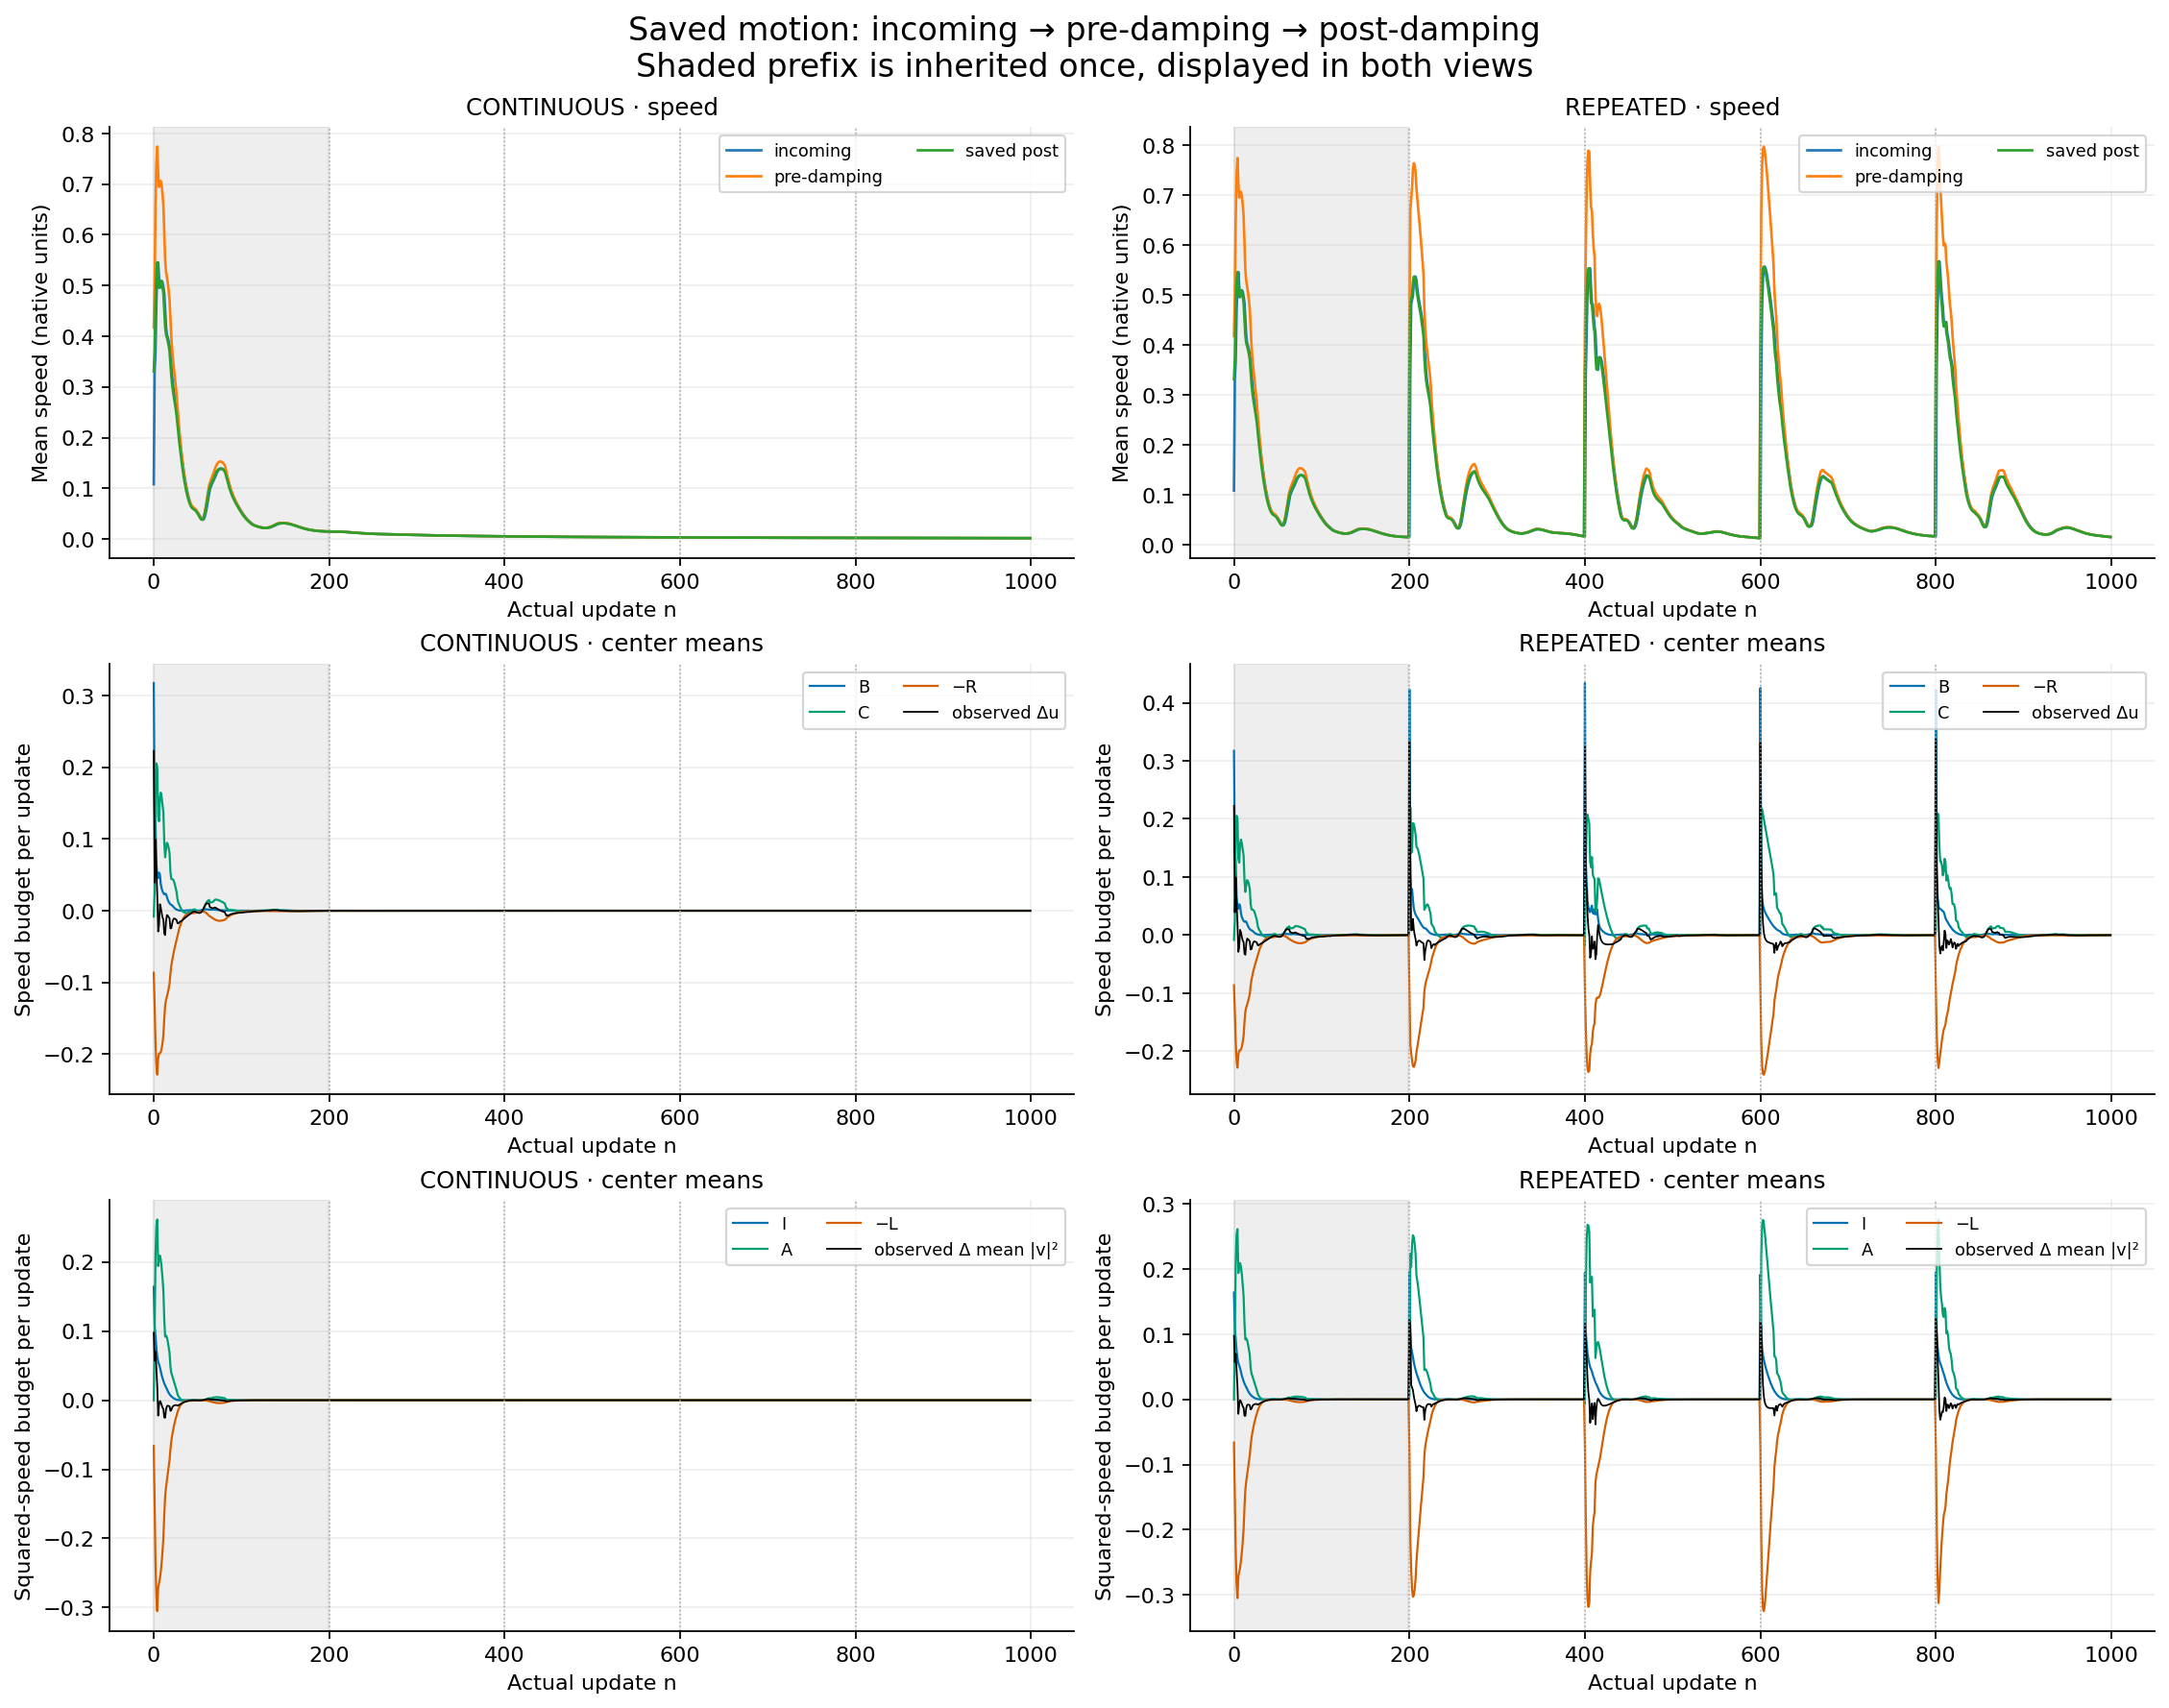
\includegraphics[width=\linewidth]{plots/01_actual_speed_budgets.png}
\caption{\small Accepted actual-update budgets, unchanged. The inherited 200-update prefix is shaded and displayed in both arms but counted once; the remaining 800 updates in each arm are SIM02 continuations. Incoming, pre-damping and post-damping speed are distinct. Repeated cycles are correlated history segments, not replicate trials.}
\label{fig:actual}
\end{figure}

The lower panels retain squared-speed units, while the middle panels directly explain changes in the upper speed curves. Recurring drive in \RPT\ accompanies substantial alignment and loss; \CONT\ enters weak forcing and continuing damping.

Over all 800 new \RPT\ updates, after averaging centers, the accepted means are
\begin{equation}
\begin{split}
\langle\mean B\rangle&=0.006030292736592971,\\
\langle\mean C\rangle&=0.015106632491045668,\\
\langle\mean R\rangle&=0.021136622830574416.
\end{split}
\label{eq:means}
\end{equation}
Their signed balance is about $3.0240\times10^{-7}$ per update over the complete four-cycle window~\cite{review}. This is a window-wide near balance, not phasewise equality. Moreover $B$ is not a causal drive-only effect: its denominator $m+r$ depends on retained state and the applied increment.

\clearpage
\section{A repeated envelope does not fix its component balances}
\label{sec:phasebudgets}
\begin{figure}[ht]
\centering
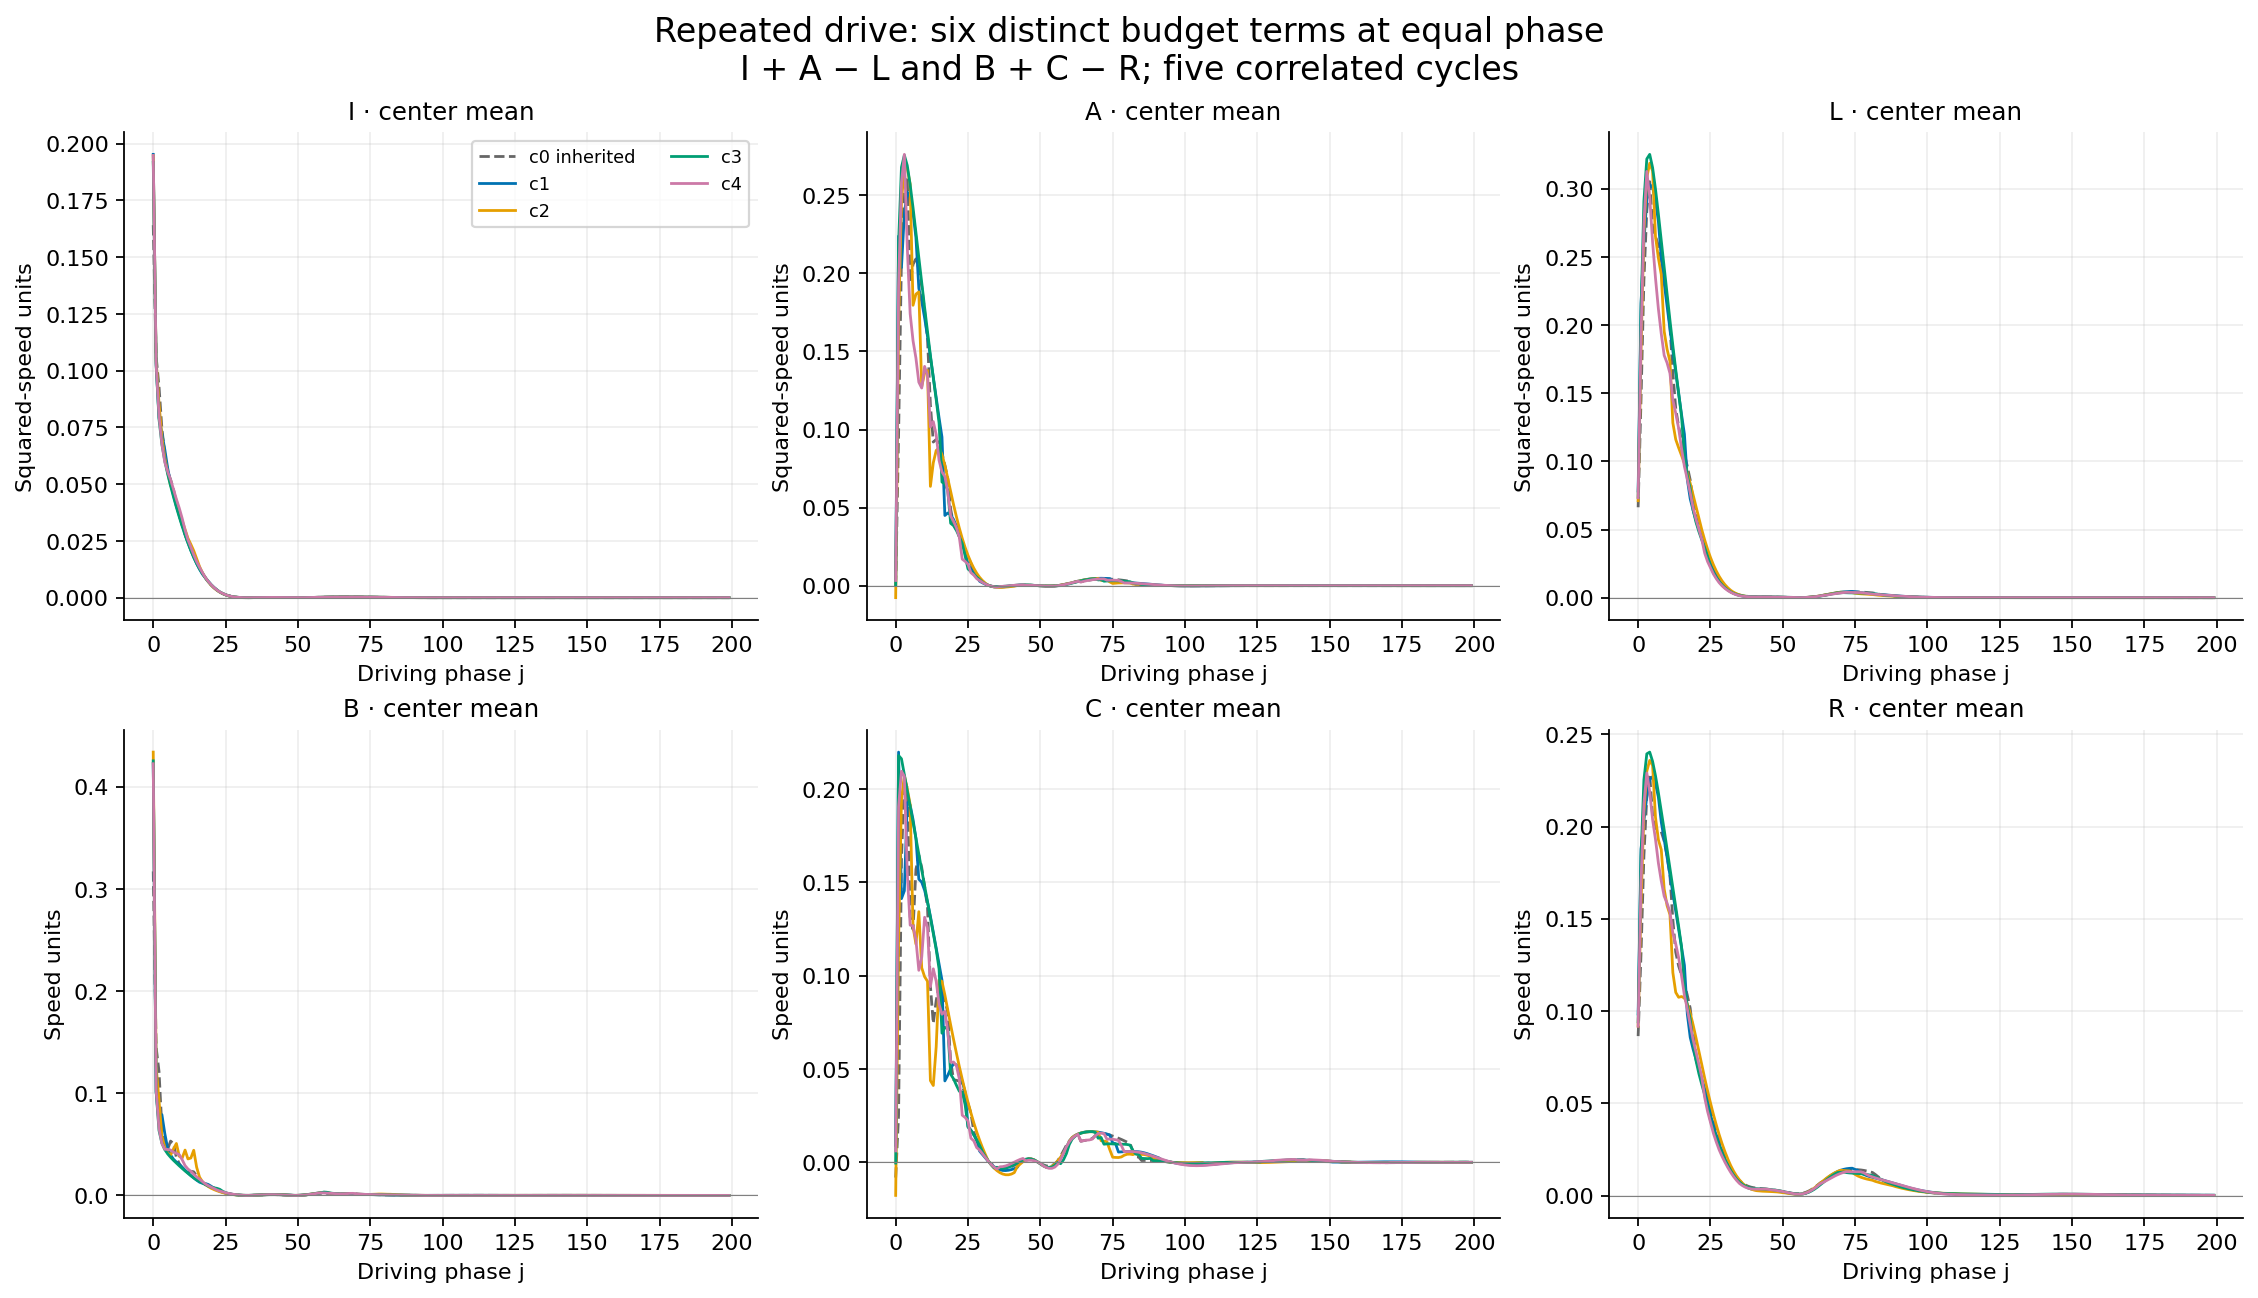
\includegraphics[width=\linewidth]{plots/02_phase_budget_terms.png}
\caption{\small Accepted phase-aligned budgets, unchanged. Dashed cycle 0 is inherited; cycles 1--4 are the new \RPT\ continuation. Each curve is a correlated history segment. $I,A,L$ have squared-speed units and $B,C,R$ speed units. Similar driving phases do not imply identical balances.}
\label{fig:phase}
\end{figure}

The new cycles receive the same source-phase schedule but have different signed speed totals. Table~\ref{tab:cycles} retains absolute alignment activity as well as signed sums. Cycle telescoping reproduces the observed boundary-speed difference; it does not establish periodic state return.
\begin{table}[ht]
\centering\small
\begin{tabular}{rrrrrr}
\toprule
Cycle & $\sum\mean B$ & $\sum\mean C$ & $\sum\mean R$ & $\sum\mean{|C|}$ & Observed $\Delta u$\\
\midrule
1 & 1.177904 & 3.172199 & 4.348652 & 3.726599 & $+0.001450748$\\
2 & 1.336903 & 2.771514 & 4.111875 & 3.946698 & $-0.003458018$\\
3 & 1.120049 & 3.299693 & 4.416184 & 3.654532 & $+0.003558535$\\
4 & 1.189379 & 2.841900 & 4.032588 & 3.255953 & $-0.001309347$\\
\bottomrule
\end{tabular}
\caption{\small Accepted new-\RPT\ cycle ledgers, rounded. Absolute activity is summed before cancellation. Full precision and all nine distinct blocks remain in the edition.}
\label{tab:cycles}
\end{table}

Across the new-four view, the RMS over phase of the population SD is $0.000416811$ for $\mean I$ and $0.00720398$ for $\mean A$; in speed units it is $0.00211627$ for $\mean B$ and $0.00772916$ for $\mean C$. These descriptive spreads retain their respective units~\cite{report}. The common impulse-magnitude structure leaves substantial state-dependent variation.

\clearpage
\section{Magnitude, regularization and the box bound}
\label{sec:q}
The source impulse separates in norm:
\begin{equation}
h_n=0.1|H_n|,\quad q_i=\frac{\norm{d_i}}{\norm{d_i}+0.01},
\quad \norm{a_i}=h_nG_nq_i,\quad
\mean I_n=h_n^2G_n^2\mean{q^2}_n.
\label{eq:factor}
\end{equation}
Signs disappear from this magnitude formula, but not from the vector increment or its alignment.
\begin{figure}[ht]
\centering
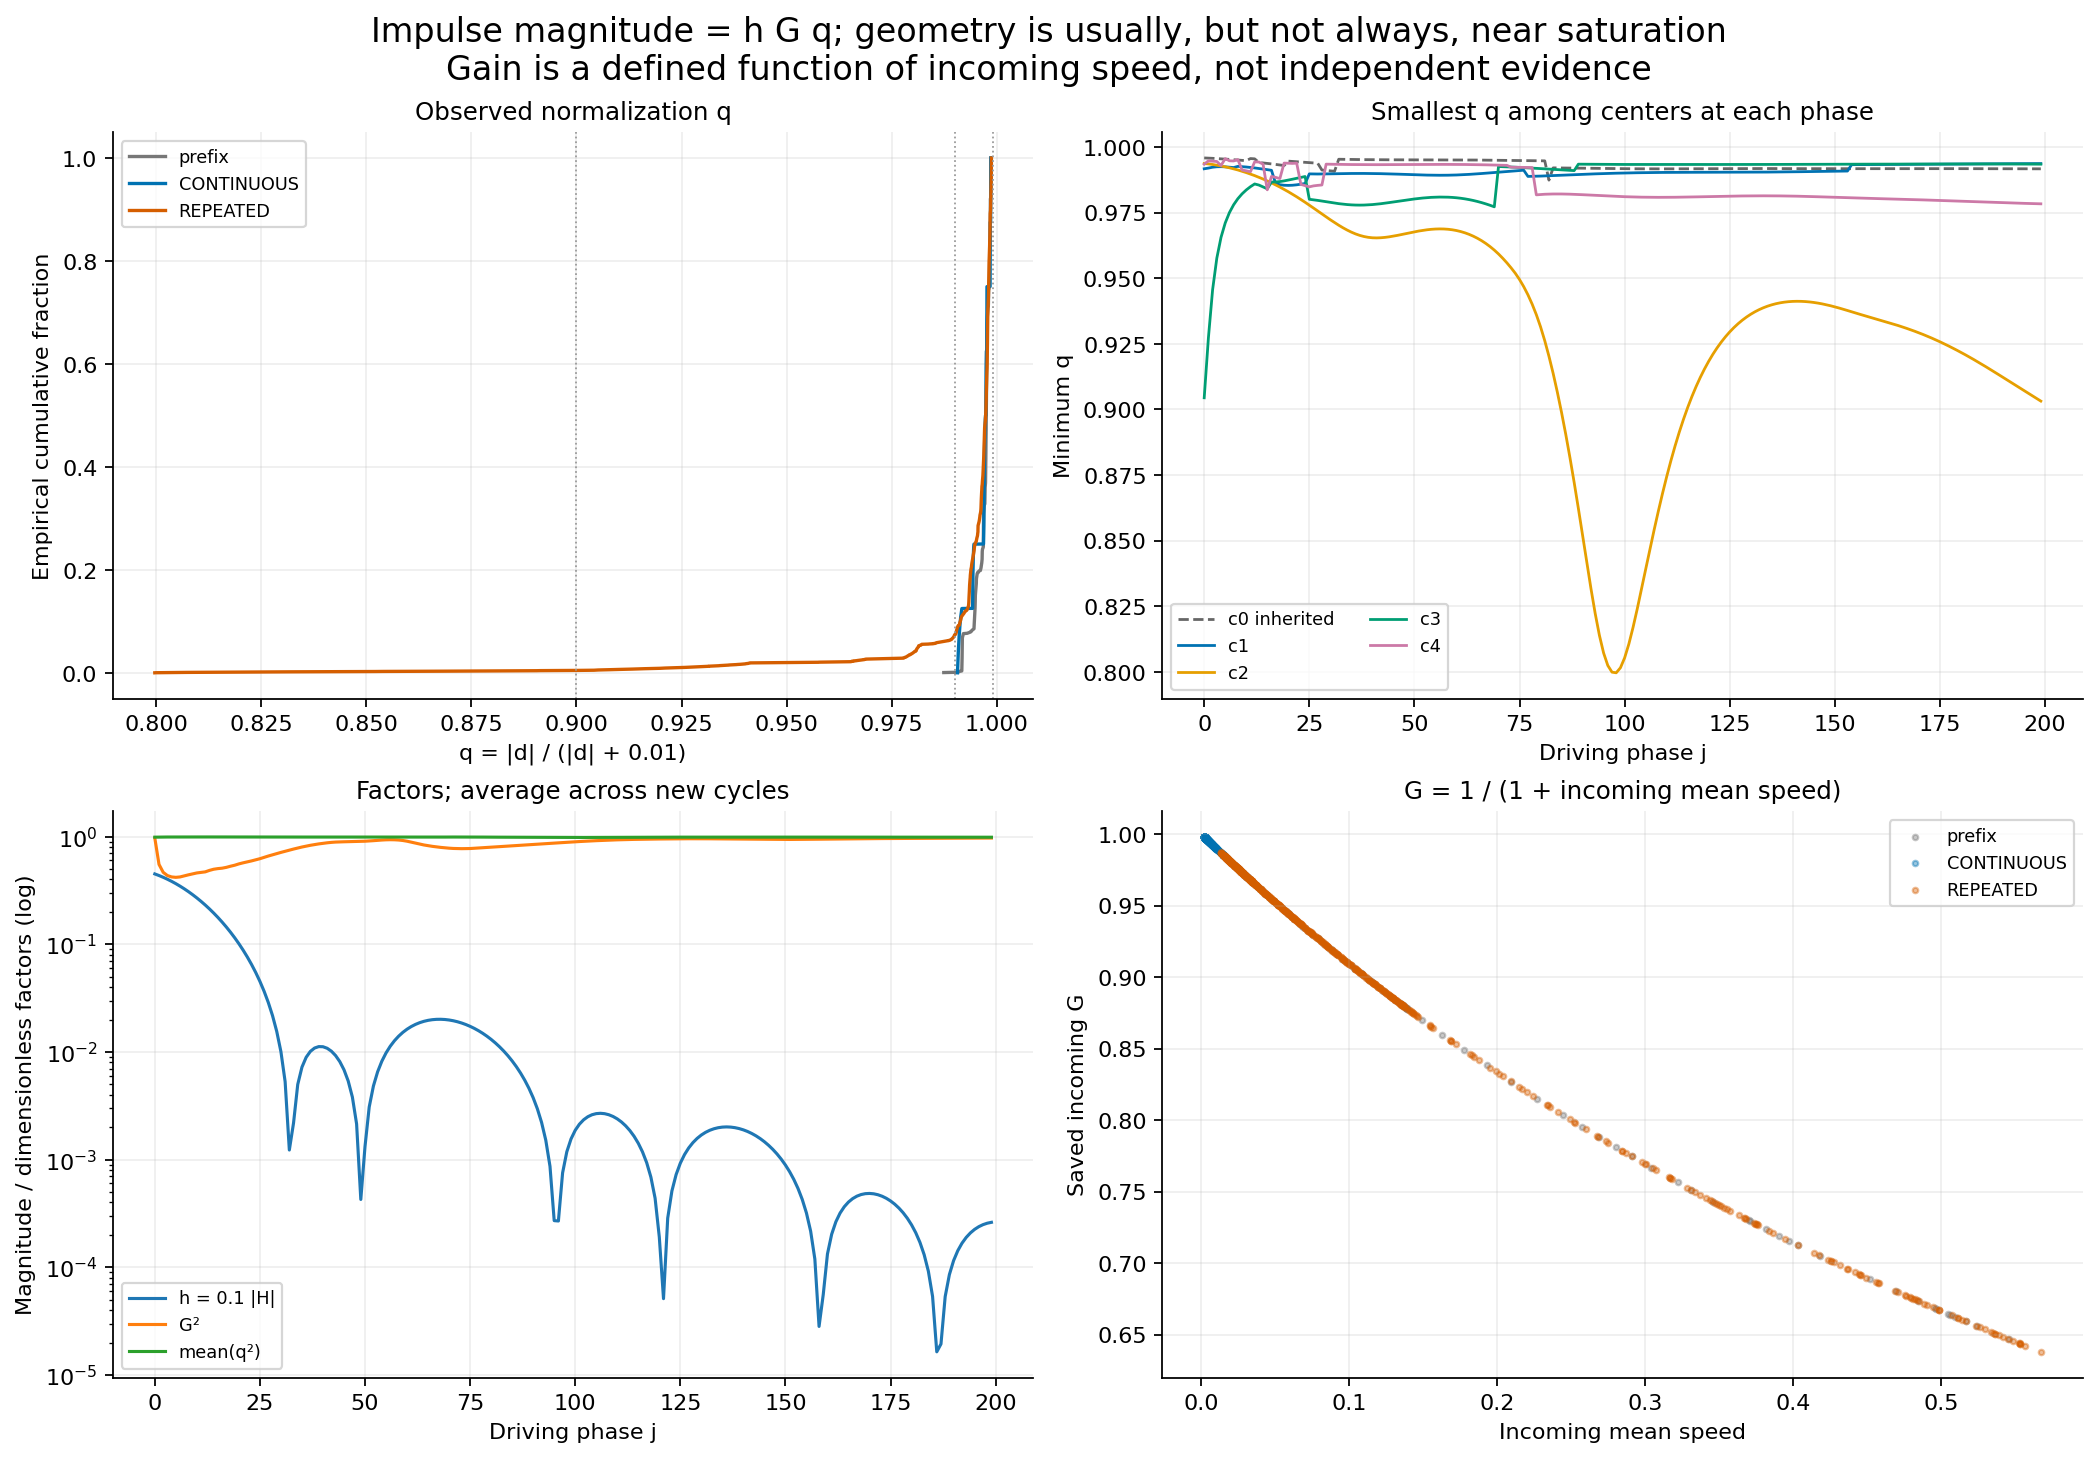
\includegraphics[width=.92\linewidth]{plots/03_normalization_and_gain.png}
\caption{\small Accepted normalization/gain diagnostics, unchanged. The inherited prefix is distinguished from the new arms and, in phase views, from cycles 1--4. Phases are correlated observations. The factor panel plots $h$, $G^2$ and mean($q^2$); the exact squared-impulse product uses $h^2$.}
\label{fig:q}
\end{figure}

$q\ge0.99$ in 96.7153\% of all center rows and 92.625\% of new \RPT\ rows. All 30 cases with $q<0.90$ occur at center 1, $n=485$--$514$. The minimum $0.7996594476$ is at $n=498$, with impulse norm about $0.0008943445$. This local suppression cannot be assigned to the strongest impulses elsewhere.

The review adds a structural limit~\cite[Sec.~5.1]{review}. Components of $d$ have magnitude at most 5, and $q$ is increasing in $\norm d$, hence
\begin{equation}
q\le\frac{5\sqrt3}{5\sqrt3+0.01}
=0.9988466312571291\ldots<0.999.
\label{eq:qbound}
\end{equation}
The zero count above 0.999 is required by the box and regularizer, not a trajectory-specific failure. Lower thresholds and localized exceptions remain informative.

\clearpage
\section{Alignment can reinforce or oppose retained motion}
\label{sec:alignment}
For nonzero $v,a$,
\begin{equation}
\cos\theta=\frac{v\cdot a}{\norm v\,\norm a},
\qquad A=2r\norm a\cos\theta,\qquad C=\frac{A}{m+r}.
\label{eq:alignment}
\end{equation}
Similar impulse norms can make opposite contributions. Geometry enters through direction as well as $q$. A large cosine with a minute impulse is not a large speed contribution.
\begin{figure}[ht]
\centering
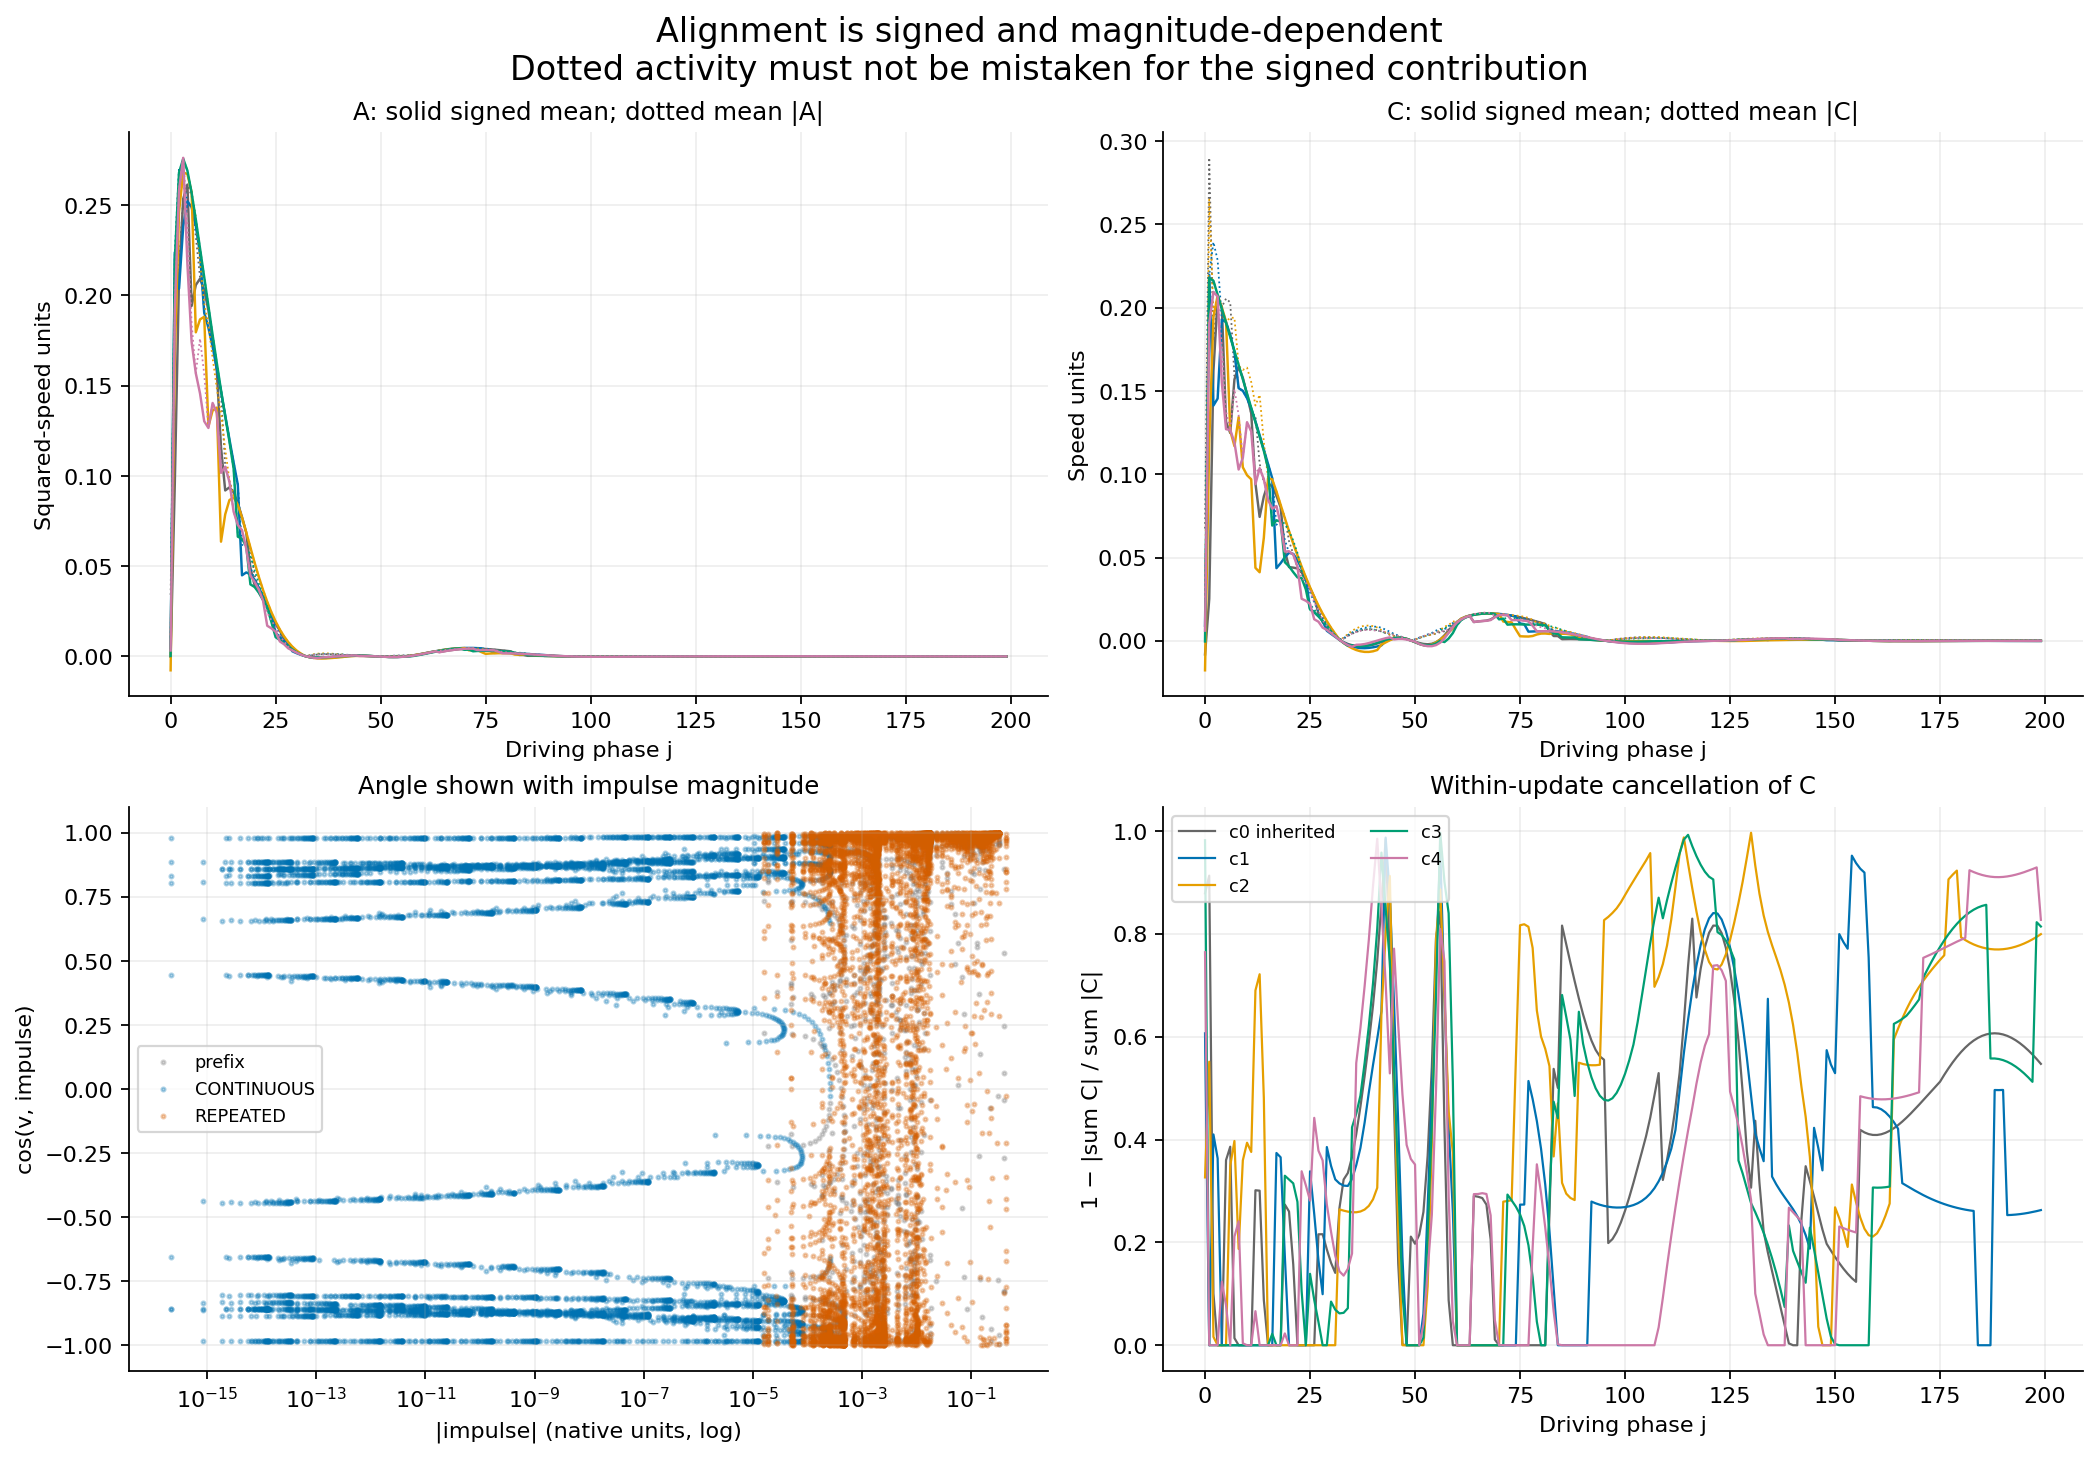
\includegraphics[width=.94\linewidth]{plots/04_alignment_and_cancellation.png}
\caption{\small Accepted alignment/cancellation diagnostics, unchanged. Phase panels distinguish inherited cycle 0 from new correlated cycles 1--4. Signed means and absolute activity are separate; the angle display retains impulse magnitude. Reporting masks hide unresolved ratios, not raw contributions.}
\label{fig:alignment}
\end{figure}

Among 6,400 new \RPT\ rows, 2,227 have negative alignment. Totals are $\sum A=102.3679$ versus $\sum|A|=109.0913$, and $\sum C=96.68245$ versus $\sum|C|=116.6703$. Aggregate cancellation fractions are about 0.0616315 and 0.171319, including cancellation across time and centers. The diagnostic is
\begin{equation}
\mathcal K_X=1-\frac{|\sum X_i|}{\sum|X_i|},\qquad X=A\text{ or }C,
\label{eq:cancellation}
\end{equation}
for a positive denominator. Zero is undefined, not perfect cancellation. A separate $10^{-12}$ reporting floor masks 294 update-level $A$ ratios and 115 $C$ ratios in weakly forced \CONT, but none in the prefix or new \RPT\ rows. No budget is divided by its nearly cancelling net change.

\clearpage
\section{The precise damping theorem}
\label{sec:theorem}
For scalar $D(x)=x/[1+\log(1+|x|)]$, put $s=|x|$. Away from zero,
\begin{equation}
D'(x)=\frac{1+\log(1+s)-s/(1+s)}{[1+\log(1+s)]^2}.
\label{eq:derivative}
\end{equation}
At zero, the difference quotient tends to 1, so $D'(0)=1$. The numerator is positive since $1-s/(1+s)>0$. Denominator minus numerator is
\[
\log(1+s)+\log^2(1+s)+s/(1+s)\ge0.
\]
Thus $0<D'(x)\le1$. Applying the scalar mean-value inequality to each coordinate and summing squares proves
\begin{equation}
\norm{D(w)-D(\widetilde w)}_2\le\norm{w-\widetilde w}_2.
\label{eq:nonexpansion}
\end{equation}

This is nonexpansion of \emph{fixed pre-damping vectors}. It is not a contraction theorem for the complete C update. Before damping, geometry and bits determine directions, gain depends on incoming velocities, and forcing can enlarge differences. Position wrapping and the sequential centroid also lie outside the theorem. There is no uniform factor below one near zero, since $D'(0)=1$.

\subsection{Scalar-speed dispersion is a different question}
Componentwise damping is not rotation invariant. Two vectors with the same norm $r>0$ give
\begin{align}
\norm{D((r,0,0))}&=\frac{r}{1+\log(1+r)},\nonumber\\
\norm{D\left(\frac r{\sqrt3}(1,1,1)\right)}
&=\frac{r}{1+\log(1+r/\sqrt3)}.
\label{eq:orientationexample}
\end{align}
Their outgoing norms differ. Even zero incoming dispersion of norms need not remain zero. This analytic distinction was checked in SIM03 and subsequently reviewed; no recorded trajectory was rotated.

The theorem controls a vector distance containing directional information. Collective mean speed discards that information before its across-cycle variance is formed. Its behavior must be measured separately, not inferred from Eq.~\eqref{eq:nonexpansion}.

Two descriptive readouts retain magnitude and orientation information:
\begin{equation}
\eta_i=\frac{\norm{D(w_i)}}{\norm{w_i}},\qquad
\chi_i=\frac{\sum_\alpha w_{i,\alpha}^4}{(\sum_\alpha w_{i,\alpha}^2)^2},
\qquad \frac13\le\chi_i\le1.
\label{eq:retention}
\end{equation}
They are defined only for nonzero $w_i$. They are not new complexity or memory measures.

\clearpage
\section{Retention and observational strata}
\label{sec:retention}
\begin{figure}[ht]
\centering
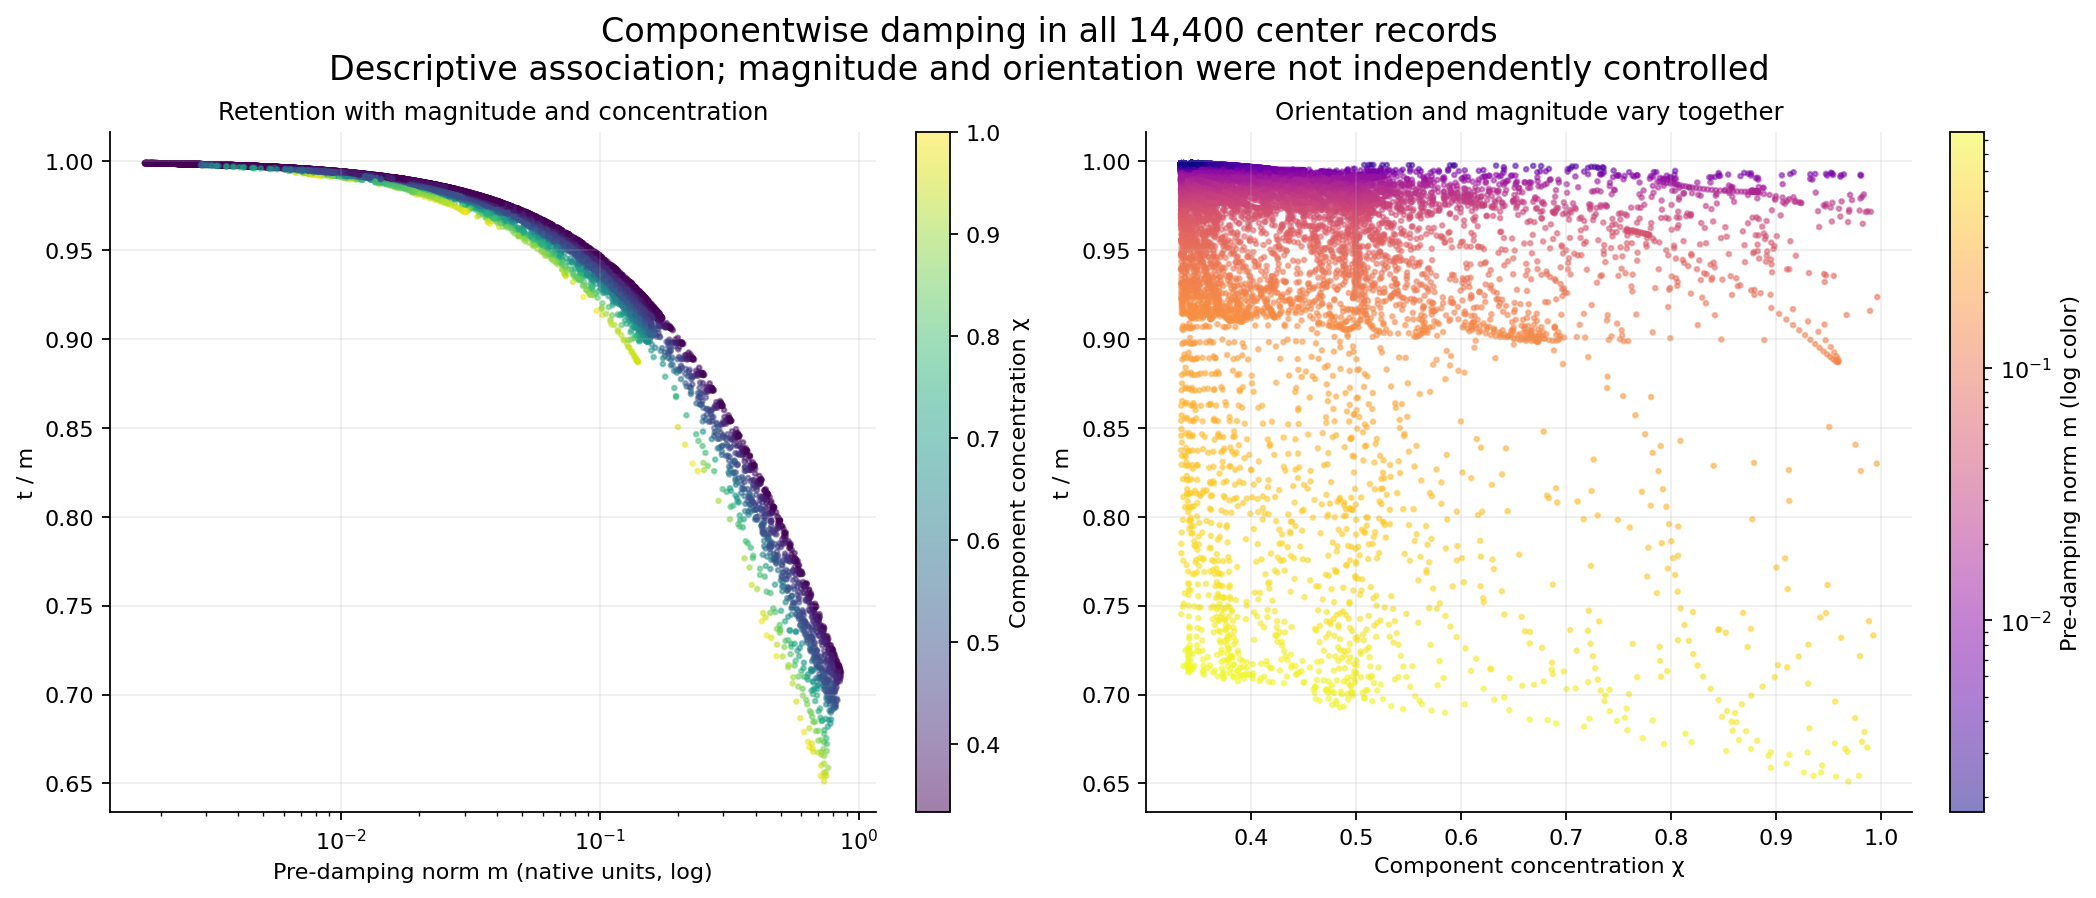
\includegraphics[width=\linewidth]{plots/05_damping_retention_orientation.png}
\caption{\small Accepted retention/orientation display, unchanged. It pools the inherited prefix once and the two new arms, 14,400 center rows. Repeated-cycle rows remain correlated. Magnitude and component concentration vary together; color separation does not isolate an orientation effect.}
\label{fig:retention}
\end{figure}

Retention spans $0.651157\ldots0.998986$ and $\chi$ spans $0.333333557\ldots0.996537$. For new \RPT\ rows, median $m$ is $0.0412528$ and retention $0.974453$; for new \CONT\ rows they are $0.00330577$ and $0.998069$. Weaker damping at small magnitude is consistent with $D'$ approaching one, but pooled medians are not controlled comparisons.

The accepted joint table uses fixed magnitude boundaries $0,.01,.05,.1,.25,.5,1,\infty$ and concentration boundaries $1/3,.45,.6,.8,1$. All 28 bins remain, including four empty bins at $m\ge1$. Within $0.25\le m<0.5$, mean retention is $0.832506$ in the lowest concentration bin and $0.763123$ in the highest. Their mean magnitudes differ, $0.374305$ versus $0.409515$, preventing an isolated causal interpretation.

\begin{table}[ht]
\centering\small
\begin{tabular}{lrrr}
\toprule
All-record stratum & Center rows & Mean $A$ & Mean $C$\\
\midrule
$H>0$ & 8,416 & $0.01514877$ & $0.01441040$\\
$H<0$ & 5,984 & $-0.0000234244$ & $-0.000244641$\\
$H=0$ & 0 & undefined & undefined\\
Bit changed & 164 & $-0.01358054$ & $-0.02276277$\\
Bit unchanged & 14,236 & $0.00910221$ & $0.00867849$\\
\bottomrule
\end{tabular}
\caption{\small Accepted observational strata. Sign and bit strata overlap and must not be added as disjoint populations. Empty strata are not zero-valued measurements.}
\label{tab:strata}
\end{table}

Saved bit changes total 14 in the prefix and 75 in each new arm. In \RPT, mean $C$ is $-0.0312923$ on changed-bit rows and $+0.0156568$ on unchanged rows. Different phases, velocities and geometry accompany these rows; this is not a bit-toggle intervention.

\clearpage
\section{Incoming, pre-damping and post-damping vector differences}
\label{sec:vectorresults}
\begin{figure}[ht]
\centering
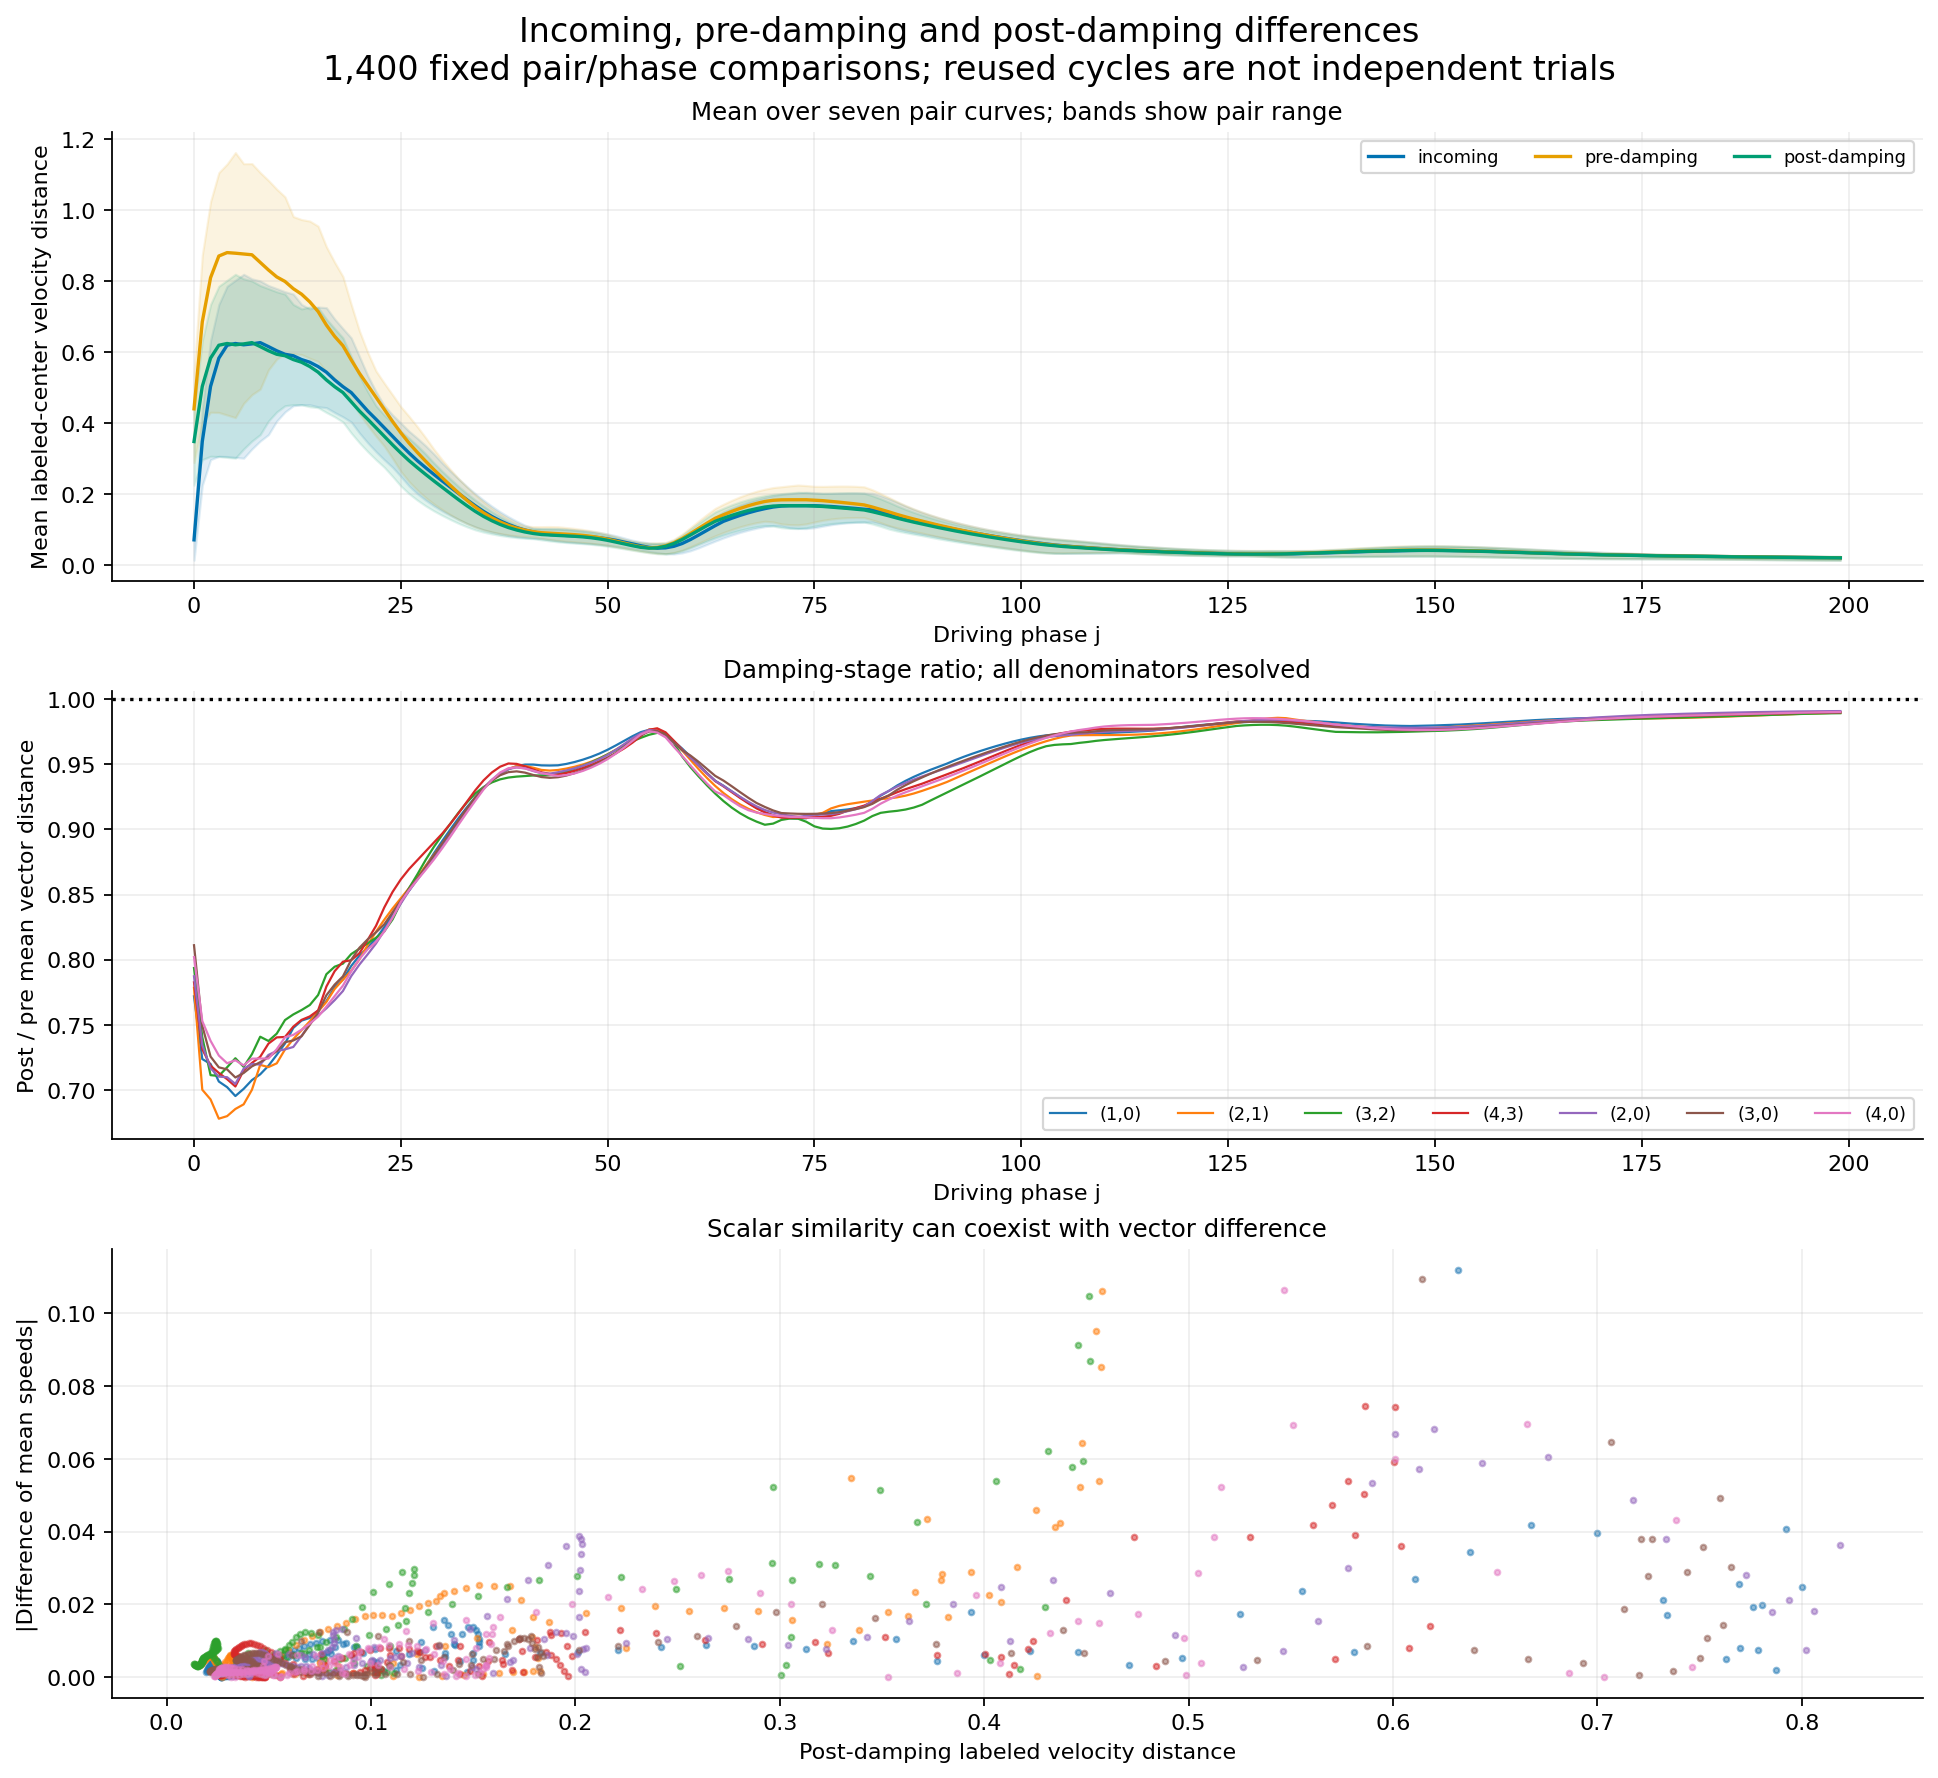
\includegraphics[width=.84\linewidth]{plots/06_phase_velocity_differences.png}
\caption{\small Accepted same-phase comparisons, unchanged. The seven pairs compare new cycles to inherited cycle 0 and to other new cycles. Bands span correlated pair curves, not confidence intervals. Incoming, pre-damping and saved post-damping vectors are separate stages; scalar-speed differences are a separate readout.}
\label{fig:vectors}
\end{figure}

All 11,200 requested center damping comparisons decrease. The largest signed post-minus-pre excess is $-1.28905\times10^{-5}$, at pair $(4,3)$, phase 138, center 0. Across 1,400 pair/phase rows, the ratio of mean post distance to mean pre-damping distance ranges from $0.678176$ to $0.990632$, with no masks.

Forcing nevertheless increases mean labeled distance from incoming to pre-damping in 134--154 of 200 phases per pair. Phase-averaged incoming/pre/post distances are $0.143332/0.175005/0.142867$ for $(1,0)$ and $0.133162/0.158424/0.133211$ for $(4,3)$. Damping-stage contraction can coexist with outgoing distance exceeding incoming distance. All pairs' mean, maximum and RMS center distances remain in the evidence~\cite{report}.

\clearpage
\section{A measured reduction of scalar-speed dispersion}
\label{sec:scalar}
Let $u_{\pre}$ be mean $\norm w$, not the incoming speed used by $G$. Since $u_{\post}=u_{\pre}-\mean R$, population moments across cycles at fixed phase obey
\begin{equation}
\Var_c(u_{\post})=\Var_c(u_{\pre})+\Var_c(\mean R)
-2\Cov_c(u_{\pre},\mean R).
\label{eq:variance}
\end{equation}
This is a descriptive identity, not causal attribution.
\begin{figure}[ht]
\centering
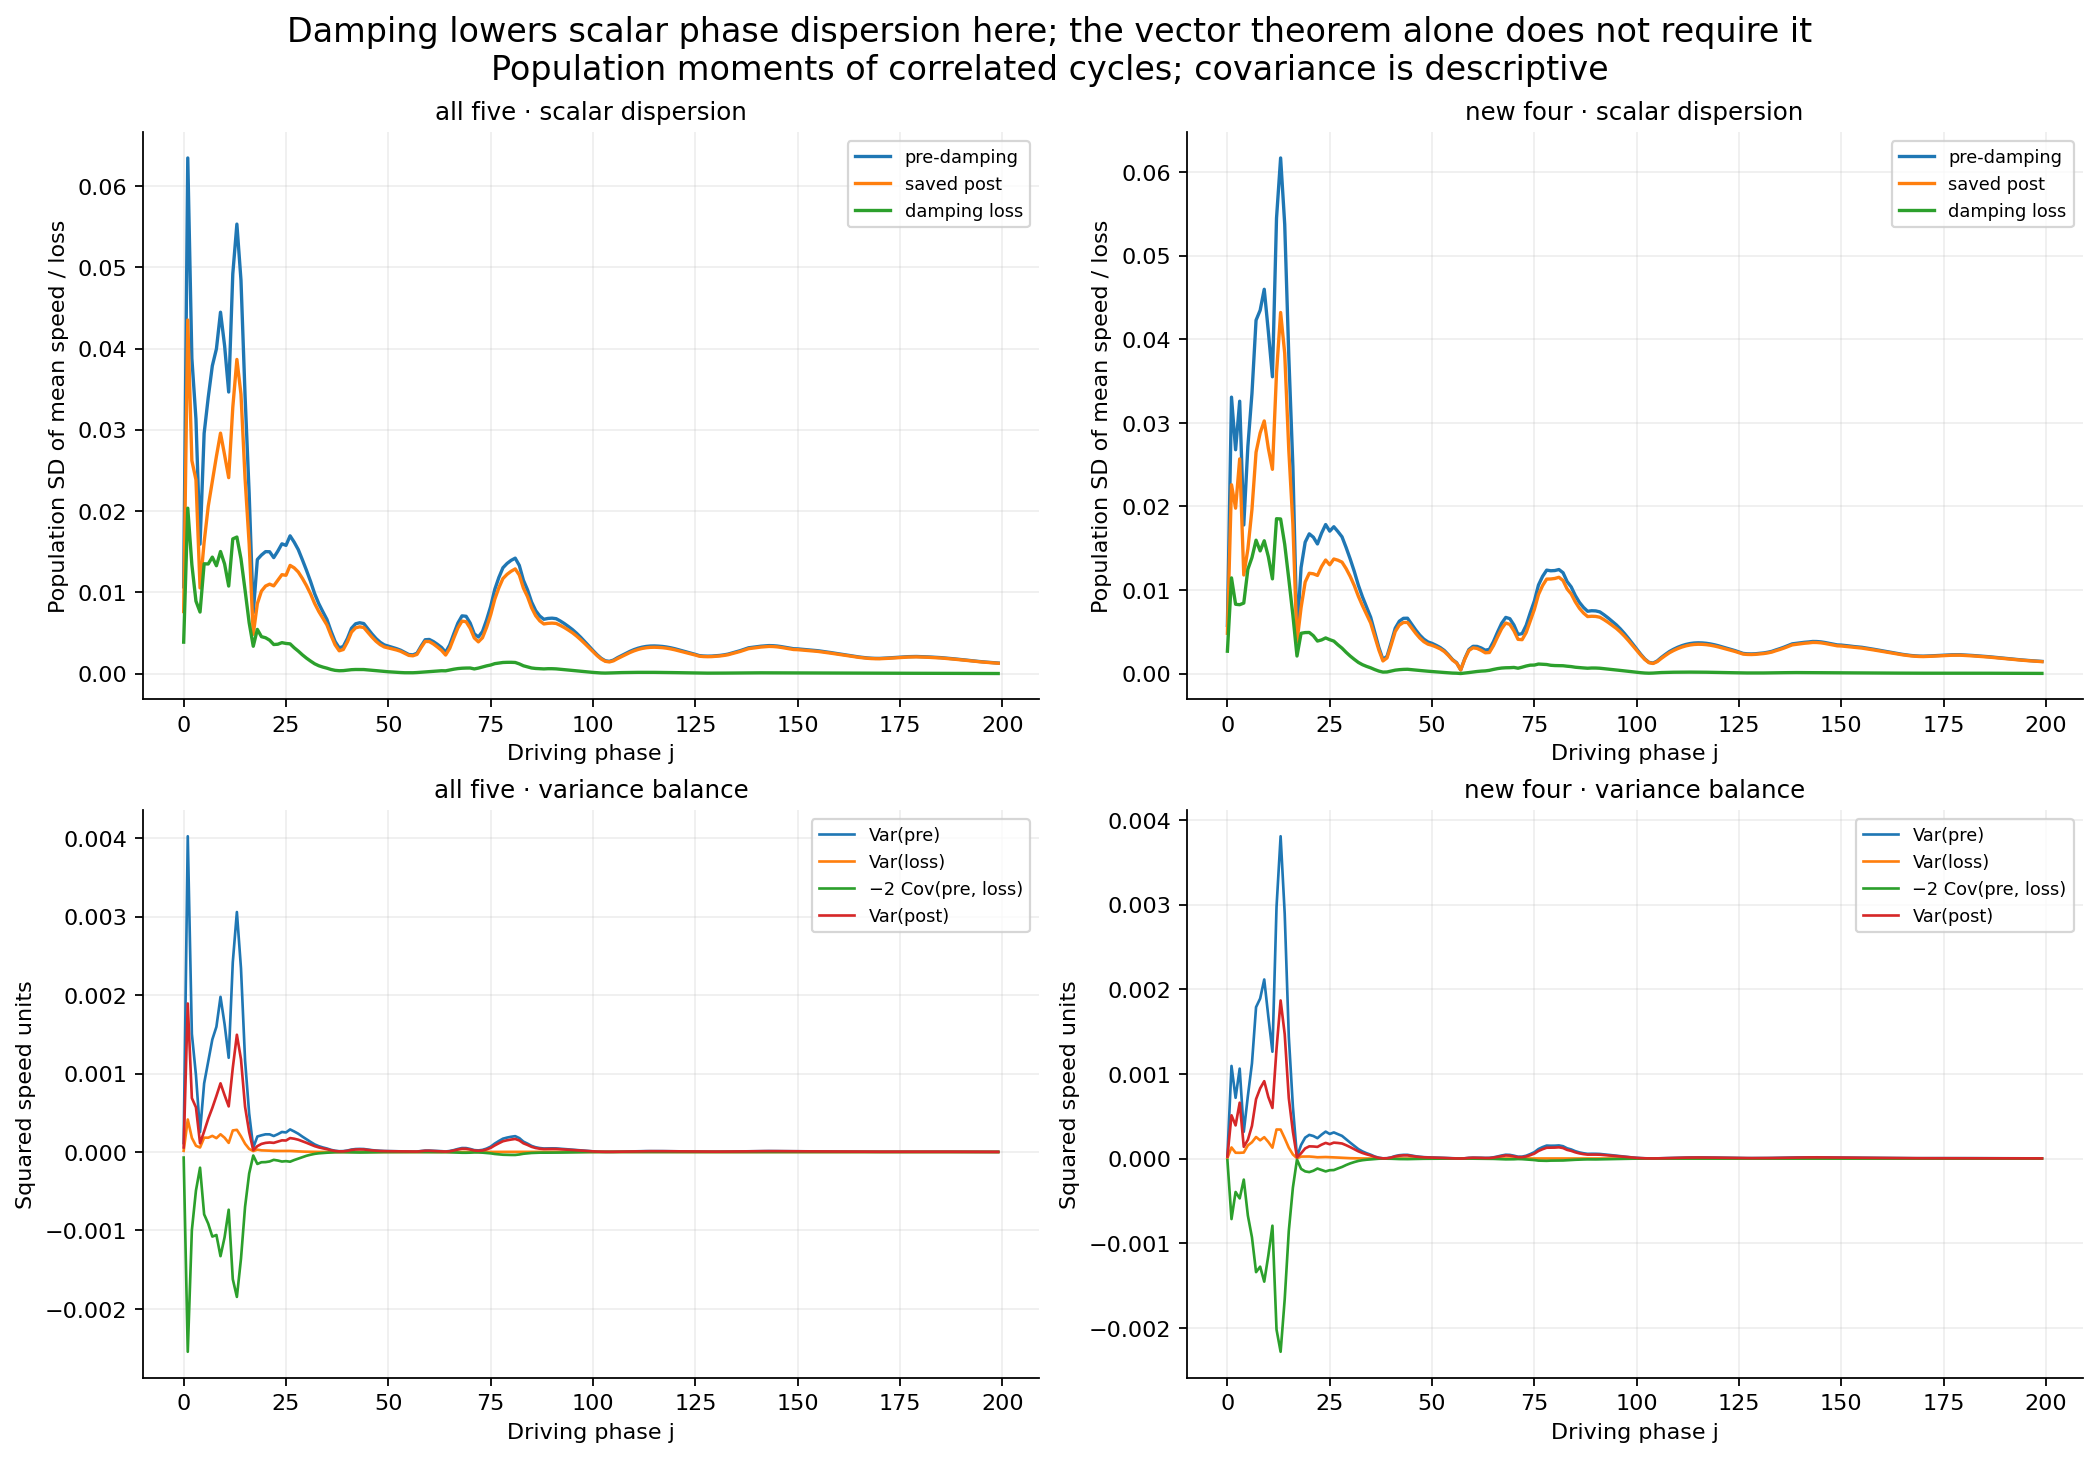
\includegraphics[width=.92\linewidth]{plots/07_scalar_dispersion_balance.png}
\caption{\small Accepted scalar dispersion/balance, unchanged. All five includes inherited cycle 0; new four uses cycles 1--4. These are population moments of correlated cycles. The measured reduction is pre-damping to post-damping, not the nearly reindexed incoming/outgoing average.}
\label{fig:variance}
\end{figure}

Variance decreases at all 200 phases in both views. Reviewer-verified smallest pre-minus-post margins are about $6.0038\times10^{-8}$ (all five) and $9.8412\times10^{-9}$ (new four). New-four phase-averaged moments are:
\begin{center}\small
\begin{tabular}{lr}
\toprule
$\langle\Var(u_{\pre})\rangle_j$ & $0.0001645312375633206$\\
$\langle\Var(\mean R)\rangle_j$ & $0.0000154319706178890$\\
$\langle\Cov(u_{\pre},\mean R)\rangle_j$ & $0.0000472054358490594$\\
$\langle\Var(u_{\post})\rangle_j$ & $0.0000855523364830908$\\
\bottomrule
\end{tabular}
\end{center}
The roughly 48.0\% decrease describes this stage-specific comparison~\cite[Sec.~4.4]{review}, not a causal fraction or future-cycle theorem. Positive covariance records how loss accompanies excess pre-damping response.

\clearpage
\section{The indexing constraint on incoming and outgoing spread}
\label{sec:indexing}
The subsequent reviewer identified a constraint on another comparison~\cite[Sec.~5.2]{review}. Fix a cycle-index set $\mathcal C$ and let $x_{c,j}=u(S_{200c+j})$. For $j<199$, outgoing speed at phase $j$ equals incoming speed at $j+1$. Therefore,
\begin{equation}
\begin{split}
&\frac1{200}\sum_{j=0}^{199}\left[
\Var_{c\in\mathcal C}u(S_{200c+j+1})
-\Var_{c\in\mathcal C}u(S_{200c+j})\right]\\
&\qquad=\frac{\Var_{c\in\mathcal C}u(S_{200(c+1)})
-\Var_{c\in\mathcal C}u(S_{200c})}{200}.
\end{split}
\label{eq:telescoping}
\end{equation}
The proof is cancellation of adjacent phase terms. Only cycle-boundary variances survive. It invokes no dynamical stability property.

\begin{table}[ht]
\centering\small
\begin{tabular}{lrrr}
\toprule
Cycle set & Incoming & Pre-damping & Post-damping\\
\midrule
All five, $0$--$4$ & 0.0096040646 & 0.0128717164 & 0.0092360174\\
New four, $1$--$4$ & 0.0092494558 & 0.0128269730 & 0.0092494506\\
\bottomrule
\end{tabular}
\caption{\small RMS over 200 phases of the population SD of actual mean speed. This RMS of phasewise SDs is not an RMS-speed replacement for the underlying observable.}
\label{tab:spread}
\end{table}

For the new-four view, phase-averaged outgoing minus incoming variance is approximately $-9.5537351\times10^{-11}$. The review found agreement with the boundary expression to about $5.2\times10^{-21}$. Most samples in the two averages are the same scalar trajectory values shifted by one update.

The near equality in Table~\ref{tab:spread} is therefore not independent evidence of self-regulation, perfect cycle stabilization or convergence. The all-five view obeys the same identity with a larger boundary contribution involving the inherited initial state.

This caveat does not remove the damping-stage observation. Pre-damping mean norm is a distinct intermediate, not merely the incoming scalar series shifted one update. Its variance is directly compared with that of the saved outgoing state. Equation~\eqref{eq:variance} and the 200/200 reductions remain separate results.

Nor is scalar resemblance exact: new-four post-speed population SD reaches $0.0432153$ at phase 13, and its mean phase range is $0.0154752$. Similar envelopes coexist with meaningful scalar differences and larger labeled-vector differences.

\clearpage
\section{The continuous arm and the dependent gain}
\label{sec:context}
\begin{figure}[ht]
\centering
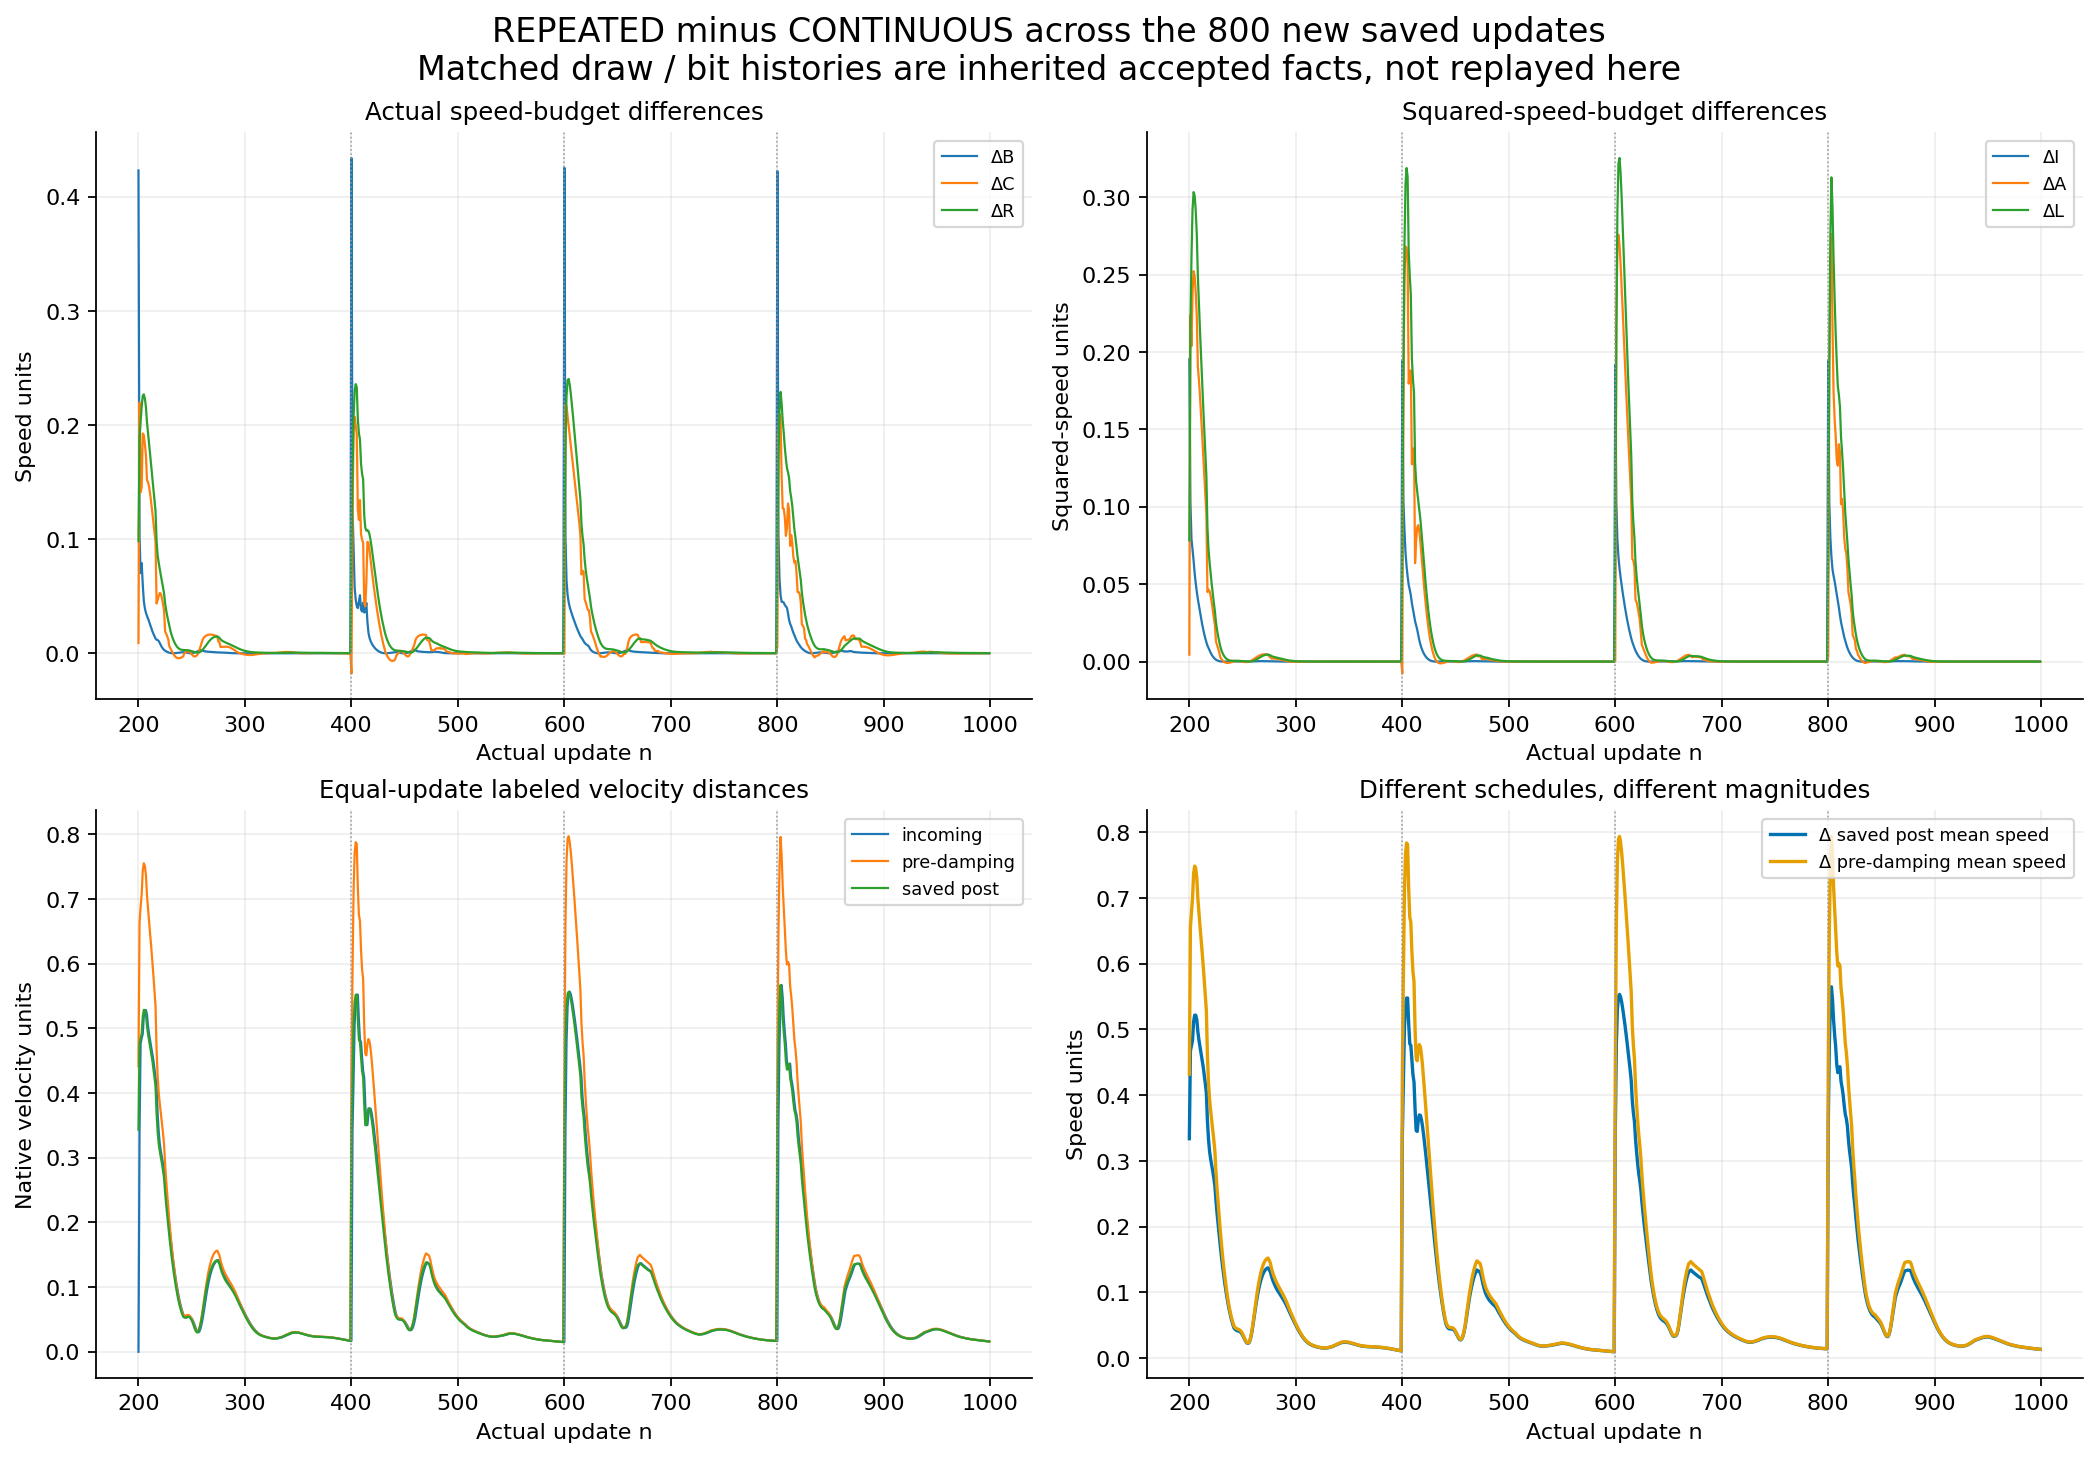
\includegraphics[width=.94\linewidth]{plots/08_cross_arm_context.png}
\caption{\small Accepted cross-arm context, unchanged. Each row is \RPT\ minus \CONT\ at equal actual $n=200,\ldots,999$, after their common inherited prefix. Only new continuations enter the differences. Repeated phases remain correlated. SIM02 changed only the supplied-frame schedule; the present decomposition does not isolate the contributions of individual internal mechanisms.}
\label{fig:cross}
\end{figure}

Over new \CONT\ updates, mean speed terms are approximately $B=3.55\times10^{-8}$, $C=1.45\times10^{-6}$ and $R=1.78\times10^{-5}$. Mean post-speed differences (\RPT\ minus \CONT) in the four blocks are $0.0951350$, $0.0943893$, $0.102233$ and $0.0984275$. All 6,400 cross-arm center pairs satisfy damping nonexpansion; the largest signed excess is $-6.90239\times10^{-6}$~\cite{report,review}.

Similar gains provide no independent explanation. Subtraction of reciprocals in Eq.~\eqref{eq:gain} gives
\begin{equation}
|G(u)-G(\widetilde u)|=
\frac{|u-\widetilde u|}{(1+u)(1+\widetilde u)}
\le|u-\widetilde u|,\qquad u,\widetilde u\ge0.
\label{eq:gaindifference}
\end{equation}
Measured $G,G^2$ are instantaneous multipliers at a recorded state, not outcomes of switching feedback off. Gain--speed correlation is built into the definition; it cannot count as statistically independent evidence of a collective mechanism.

\clearpage
\section{Verification, interpretation and limits}
\label{sec:limits}
The accepted Windows analysis matched all 43,200 saved successor components exactly in its executed environment. Its largest center budget residual was $2.220446049250313\times10^{-16}$; largest block-telescoping residual was about $5.27\times10^{-16}$. Tolerances remained $10^{-12}$ for center/update relations and $10^{-10}$ for block telescoping~\cite{qa}. No unmasked nonfinite primary value occurred.

GPT's internal review used another platform and numerical stack. Maximum velocity residuals were $1.1102230246251565\times10^{-16}$ for prefix and \RPT, and $1.734723475976807\times10^{-18}$ for \CONT. This is cross-environment numerical consistency, not bitwise equivalence~\cite{review}.

\begin{table}[ht]
\centering\small
\begin{tabular}{lrrr}
\toprule
Work & Distinct updates & Reconstruction evaluations & New updates\\
\midrule
SIM03 analysis & 1,800 & 1,800 & 0\\
GPT review & 1,800 & 3,600 over two attempts & 0\\
Manuscript preparation & no added population & 0 & 0\\
\bottomrule
\end{tabular}
\caption{\small Scientific analysis and later checking are separately counted. Repeated review and display do not create independent trajectories.}
\label{tab:accounting}
\end{table}

The first reviewer attempt stopped at a normalized signed-mean ratio whose small denominator amplified rounding differences. The second retained the quotient discrepancy and checked that ratio times absolute mean equals population SD at unchanged native-unit tolerance. It passed. Both attempts remain disclosed: 28,800 center and 86,400 component evaluations over the same distinct population~\cite{reviewaccount}. Accepted values were not rewritten.

The supported explanation combines repeated magnitude structure, usually weak distance suppression, substantial signed alignment and damping that compresses differences at its own stage in these records. It does not isolate individual causal effects. It establishes no universal response shape, learned memory, shape-invariant recurrence, physical energy conservation, new topology, fixed point or asymptotic attractor theorem.

C is not established as the missing June full-constant producer. An informal convention of normalizing a total near 13.8 to 1 is not evidence for changing C's box length, inserting $\pi,e,\phi$ or rescaling its dynamics. Accepted source and observations remain the subject.

A remaining question concerns explicit conditions under which the coupled forcing--damping update bounds phasewise collective-speed dispersion. That separate investigation is not performed here. The contribution is the exact finite observed-path decomposition and its separated mathematical and empirical implications.

\clearpage
\section*{Data, source access and assistance}
The edition retains the accepted report, eight original PNGs, ten analysis CSVs, two derived NPZ files, results, selected QA records, source definitions, three saved-state records and the seven-member subsequent GPT review. The claim-source map connects equations, figures, quantitative claims and reviewer clarifications to preserved records.

The access guide distinguishes the curated edition from the full original submission. Workstation-oriented helpers and private closeout receipts are omitted rather than silently redacted. Analyst/reviewer scripts are inspection material; this subset is not a turnkey execution package. The research adds no runtime authority to the Tri-Octagon kernel or UI.

Hilmir Frímann Halldórsson is the human research author. GPT provided scientific direction and subsequent internal review; Codex performed passive-analysis implementation and manuscript engineering. These are assistance credits, not AI coauthorship, external peer review or independent laboratory validation. No affiliation, funding award, DOI or new licence is claimed. Repository software licensing does not automatically license this research.

\begin{thebibliography}{9}\small\raggedright
\bibitem{sim01}
H.~F.~Halldórsson, \emph{Early SRG Recursive Motion: Source Reconstruction, Stateful Feedback, and Finite Replays}, SIM01 research note, v0.1 (2026).
\href{https://github.com/pzychozen/trioctagon-physics/blob/0ecedec5a7d7077740b0d336ba9959dc8f117caf/SRG_REDISCOVERY/SIM01_SURVIVING_RECURSIVE_MOTION/publication/v0.1/README.md}{Pinned SIM01 edition}.
\bibitem{sim02}
H.~F.~Halldórsson, \emph{Repeated Driving and Retained State in Early SRG Motion: A Bounded Paired Continuation of Historical Engine C}, v0.1 (2026).
\href{https://github.com/pzychozen/trioctagon-physics/blob/36621a283c48edbd6050771a5beddc4dde7cedcf/SRG_REDISCOVERY/SIM02_REPEATED_DRIVE_AND_RETAINED_STATE/publication/v0.1/README.md}{Pinned SIM02 edition}.
\bibitem{source}
Historical engine C: original source, accepted detached numerical core and API. Retained under \src{inputs/accepted_sim02/inputs/}, with provenance pinned through SIM02.
\bibitem{report}
\emph{SIM03 --- Driving, geometry and response alignment}, accepted report (14 October 2026), \src{SIM03_REPORT.md}. Tables and arrays: \src{analysis/}. Submission SHA-256 begins \src{219edf82a5ad646e}; full identities appear in the edition access guide and manifest.
\bibitem{qa}
SIM03 numerical and algebra evidence, \src{evidence/QA.json} and \src{evidence/ALGEBRA_GATE.json}; implementation under \src{analyst/}. Original analysis: Python 3.11.15, NumPy 2.4.4, Windows.
\bibitem{review}
GPT, \emph{SRG-SIM03 --- GPT scientific review} (14 October 2026), \src{review/SIM03_GPT_SCIENTIFIC_REVIEW.md}. Accepted within passive mechanistic-decomposition scope without required corrections. Internal review of supplied evidence; Python 3.13.5, NumPy 2.3.5, Linux.
\bibitem{reviewaccount}
GPT review execution note and verification results, \src{review/REVIEW_EXECUTION_NOTE.json} and \src{review/INDEPENDENT_REVIEW_RESULTS.json}, unchanged. They report prior checking, not manuscript-stage execution.
\end{thebibliography}
\end{document}
